% Licensed to the Apache Software Foundation (ASF) under one or more
% contributor license agreements. See the NOTICE file distributed with
% this work for additional information regarding copyright ownership.
% The ASF licenses this file to You under the Apache License, Version 2.0
% (the ``License''); you may not use this file except in compliance with
% the License. You may obtain a copy of the License at
%
% http://www.apache.org/licenses/LICENSE-2.0
%
% Unless required by applicable law or agreed to in writing, software
% distributed under the License is distributed on an ``AS IS'' BASIS,
% WITHOUT WARRANTIES OR CONDITIONS OF ANY KIND, either express or implied.
% See the License for the specific language governing permissions and
% limitations under the License.

\documentclass[twoside]{article}
\usepackage{fullpage}
\usepackage{fancyhdr}
\usepackage{arabtex}
\usepackage{utf8}
\usepackage[utf8]{inputenc} 
\usepackage[russian,english]{babel}
\usepackage{graphicx}
\usepackage{palatino}
\usepackage{color}
\usepackage{mcstyle}
\usepackage{longtable}
\usepackage{epic}
\usepackage{hevea}
\usepackage[bookmarks=true,bookmarksnumbered=true,colorlinks=true,linkcolor=black,urlcolor=blue]{hyperref}
\usepackage{lastpage}

\setlength\parskip{\bigskipamount}
\parindent=0in

% This file contains the things that make each title page unique.
% Licensed to the Apache Software Foundation (ASF) under one or more
% contributor license agreements. See the NOTICE file distributed with
% this work for additional information regarding copyright ownership.
% The ASF licenses this file to You under the Apache License, Version 2.0
% (the ``License''); you may not use this file except in compliance with
% the License. You may obtain a copy of the License at
%
% http://www.apache.org/licenses/LICENSE-2.0
%
% Unless required by applicable law or agreed to in writing, software
% distributed under the License is distributed on an ``AS IS'' BASIS,
% WITHOUT WARRANTIES OR CONDITIONS OF ANY KIND, either express or implied.
% See the License for the specific language governing permissions and
% limitations under the License.

\newcommand{\client}{}
\newcommand{\product}{MetaCarta Appliance}
\newcommand{\doctype}{Share Connector Guide}
\newcommand{\vers}{4.5}
\newcommand{\ourlong}{MetaCarta, Inc.}
\newcommand{\authname}{Rachel Elizabeth Dillon and Malima Isabelle Wolf}
\newcommand{\theyear}{2009} 

\ShareGuidetrue
\BigMarginstrue



\ifSmallGuide
% This is a change from woody for reasons I don't fully understand.
% However, now it works.
% OK, I lied before. (How does this keep changing??)
\usepackage[twoside,hmargin={.125in, 1.185in}, twosideshift=0pt, bindingoffset=0pt]{geometry}
\flushbottom
\fi

\fancyhf{}
\fancyhead[C]{\hrule height 1.5pt \vspace{2pt}}
\fancyhead[RO,LE]{\textbf{\client\ \product\ \doctype}}
\fancyhead[LO,RE]{Version \vers}
\fancyfoot[LO,RE]{\scriptsize{{\it \copyright \theyear\ \ourlong\ All Rights Reserved. Confidential and Proprietary.}}}
\fancyfoot[RO,LE]{\scriptsize{Page \thepage\ of \pageref{LastPage}}}
\renewcommand{\headrulewidth}{0.5pt}
\renewcommand{\footrulewidth}{0.5pt}
% This has to be there to keep the text from running up into the headers.
\setlength{\headsep}{24pt}

\fancypagestyle{title}{%
\fancyhf{}
\fancyfoot[C]{\scriptsize{{\it \copyright \theyear\ \ourlong\ All Rights Reserved. Confidential and Proprietary.} \\%
Page \thepage\ of \pageref{LastPage}}}
\renewcommand{\headrulewidth}{0pt}
\renewcommand{\footrulewidth}{0pt}}
\begin{document}
\thispagestyle{title}
\begin{center}

\includegraphics[width=300pt]{mclogo}\\
{\LARGE{\textsc{\client\ \product \\
\doctype \\
\ifDraft DRAFT \\ \fi}
Last modified on \today\ \\
%\authname \\
Version \vers \\}}
\vspace{2in}

\ifInQTel
\begin{changemargin}{1in}{1in}
{\it Apache will never, ever have this conditional set.}
\end{changemargin}
\fi

\end{center}
%\begin{flushright}
%\end{flushright}

\ifDraft \pdfinfo{/DRAFT(This document is a draft, and should not be released.)} \fi
\pdfinfo{/VERSION(\vers)}

\pagebreak
\thispagestyle{title}
{\footnotesize You can put all the copyright and legalese stuff here.}
\pagebreak

\fontfamily{phv}\selectfont
\pagestyle{fancy}

%This file contains the list of includes. Even if there is only one 
%body file, we should do an include to it. 
% Licensed to the Apache Software Foundation (ASF) under one or more
% contributor license agreements. See the NOTICE file distributed with
% this work for additional information regarding copyright ownership.
% The ASF licenses this file to You under the Apache License, Version 2.0
% (the ``License''); you may not use this file except in compliance with
% the License. You may obtain a copy of the License at
%
% http://www.apache.org/licenses/LICENSE-2.0
%
% Unless required by applicable law or agreed to in writing, software
% distributed under the License is distributed on an ``AS IS'' BASIS,
% WITHOUT WARRANTIES OR CONDITIONS OF ANY KIND, either express or implied.
% See the License for the specific language governing permissions and
% limitations under the License.

% Licensed to the Apache Software Foundation (ASF) under one or more
% contributor license agreements. See the NOTICE file distributed with
% this work for additional information regarding copyright ownership.
% The ASF licenses this file to You under the Apache License, Version 2.0
% (the ``License''); you may not use this file except in compliance with
% the License. You may obtain a copy of the License at
%
% http://www.apache.org/licenses/LICENSE-2.0
%
% Unless required by applicable law or agreed to in writing, software
% distributed under the License is distributed on an ``AS IS'' BASIS,
% WITHOUT WARRANTIES OR CONDITIONS OF ANY KIND, either express or implied.
% See the License for the specific language governing permissions and
% limitations under the License.

\begin{changemargin}{1.5in}{0in}

\section{Overview}

The MetaCarta GTS appliance indexes documents and allows users
to search these documents based on both keywords and geographic
references. The MetaCarta Connector Framework allows system
administrators to configure connections to repositories and define
jobs to maintain synchronization between the repositories and the GTS
index. The Connector Framework includes five different connectors. The
Documentum Connector creates connections to EMC\circler\linebreak
Documentum\circler~repositories. The JDBC Connector creates connections
to SQL repositories, with support for Oracle\circler, Postgres SQL,
and Microsoft\circler~SQL Server\circler\linebreak (Version greater
than 6.5) repositories.  The Livelink Connector creates connections to
Open Text\circler~Livelink\circler~repositories. The Share Connector
creates connections to network shares, with full support for Microsoft
Windows\circler~shares and Samba shares, and limited support for
NetApp\circler~shares. The RSS Connector creates connections to RSS feeds.

This document specifies the means for connecting to these repositories,
indexing files from these repositories, and maintaining connections to
these repositories.

\subsection{Assumptions}

This document assumes you have a basic level of familiarity with GTS
appliance administration. This document also assumes that you have a
basic understanding of the repositories to which you are trying to
connect. If you need more information about the MetaCarta GTS
appliance, please read the \documentref{MetaCarta GTS Administrator's
Guide} stored on the appliance at
\dirpath{/usr/share/doc/metacarta/AdminGuide.pdf}. For more
information about your repositories, please see your repository
documentation or repository administrator.

Throughout this document, we assume that your appliance is named \\
\url{metacarta.example.com}. 


%What is the name of the product package? I am just calling it
% Connector Addon for now.

\section{Installation}

The Connector Framework is part of the Connector Addon available from
Metacarta. % Licensed to the Apache Software Foundation (ASF) under one or more
% contributor license agreements. See the NOTICE file distributed with
% this work for additional information regarding copyright ownership.
% The ASF licenses this file to You under the Apache License, Version 2.0
% (the ``License''); you may not use this file except in compliance with
% the License. You may obtain a copy of the License at
%
% http://www.apache.org/licenses/LICENSE-2.0
%
% Unless required by applicable law or agreed to in writing, software
% distributed under the License is distributed on an ``AS IS'' BASIS,
% WITHOUT WARRANTIES OR CONDITIONS OF ANY KIND, either express or implied.
% See the License for the specific language governing permissions and
% limitations under the License.

If you have not already installed the Connector Addon, you should use
the Connector Addon DVD to install it using the following steps:

\begin{enumerate}

\item Insert the DVD in your appliance.

\item Install the Connector Addon:

\begin{console}

metacarta:\~{}\$ sudo upgrade\_control install --from-dvd 

\end{console}

This will restart your appliance and eject the Connector Addon DVD.

\item Upgrade your license file, if necessary. For instructions,
see the \documentref{MetaCarta Appliance Administrator's Guide} or 
contact Customer Support (see page \pageref{SupportContact}).

\end{enumerate}

The Connector Addon cannot be uninstalled.

\subsection{Remote Updates}

In some cases, it may be very difficult to get physical access to an
appliance in order to install new software. To make the installation
process easier, MetaCarta provides a mechanism for remote
installations.  MetaCarta will provide you with ISO images of the
software you need upon request.  In brief, you can install the 
Connector Addon from ISO with the following command:

\begin{console}

metacarta:\~{}\$ sudo upgrade\_control install /path/to/iso.iso

\end{console}

For more information on the use of ISO
images for remote installations, see the \documentref{MetaCarta GTS
Administrator's Guide} stored on the appliance at
\dirpath{/usr/share/doc/metacarta/AdminGuide.pdf}.


\section{Configuration}

\subsection{Access to the Connector}

To use the Connector Framework, you % Licensed to the Apache Software Foundation (ASF) under one or more
% contributor license agreements. See the NOTICE file distributed with
% this work for additional information regarding copyright ownership.
% The ASF licenses this file to You under the Apache License, Version 2.0
% (the ``License''); you may not use this file except in compliance with
% the License. You may obtain a copy of the License at
%
% http://www.apache.org/licenses/LICENSE-2.0
%
% Unless required by applicable law or agreed to in writing, software
% distributed under the License is distributed on an ``AS IS'' BASIS,
% WITHOUT WARRANTIES OR CONDITIONS OF ANY KIND, either express or implied.
% See the License for the specific language governing permissions and
% limitations under the License.

must have
access to the web interface at
\url{http://metacarta.example.com/crawler/}. In the default appliance
security setup, you must have a Basic Authentication account
configured for access to the Connector web interface at
\url{http://metacarta.example.com/crawler/}.  If you are not an appliance
administrator, please ask the appliance administrator to give you such
an account.

An appliance administrator can create an account with access to the
ingestion interface (in this case, username {\tt fred} and password
{\tt ginger}) by running the following command on the appliance:

\begin{console}
metacarta:\~{}\$ basic\_auth\_control add ingest\_users fred:ginger 
\end{console}

Depending on how you have configured authentication using the
\command{auth\_control} tool, you may need to make changes other than
adding yourself to the ingest\_users group. For more information on
security configuration and \command{auth\_control}, see the Security
Administration section of the \documentref{MetaCarta Appliance
Administrator's Guide}.


\subsection{Initial Repository Configuration}

Some repositories and security models require additional configuration
to the GTS appliance. In most cases you will need to perform these
setup steps before using the crawler interface. You may need the help
of your GTS appliance administrator to complete these steps.

\subsubsection{Initial Active Directory Configuration}

The Documentum Connector, Livelink Connector, and Share Connector all
support the Active Directory security model. % Licensed to the Apache Software Foundation (ASF) under one or more
% contributor license agreements. See the NOTICE file distributed with
% this work for additional information regarding copyright ownership.
% The ASF licenses this file to You under the Apache License, Version 2.0
% (the ``License''); you may not use this file except in compliance with
% the License. You may obtain a copy of the License at
%
% http://www.apache.org/licenses/LICENSE-2.0
%
% Unless required by applicable law or agreed to in writing, software
% distributed under the License is distributed on an ``AS IS'' BASIS,
% WITHOUT WARRANTIES OR CONDITIONS OF ANY KIND, either express or implied.
% See the License for the specific language governing permissions and
% limitations under the License.

If you want to enforce Active Directory security on documents crawled
from \ifDocumentumGuide Documentum,\fi \ifLivelinkGuide Livelink,\fi
\ifShareGuide your network share,\fi \ifCombinedConnectorGuide your
repositories,\fi you must configure your appliance for Active
Directory support. Ask your administrator whether or not your
appliance is configured to use Active Directory.

For more information on this step, please see the \documentref{MetaCarta
GTS Administrator's Guide}, located on the appliance at
\dirpath{/usr/share/doc/metacarta}\linebreak\dirpath{
/AdminGuide.pdf}.


\subsubsection{Initial Documentum Configuration}

% Licensed to the Apache Software Foundation (ASF) under one or more
% contributor license agreements. See the NOTICE file distributed with
% this work for additional information regarding copyright ownership.
% The ASF licenses this file to You under the Apache License, Version 2.0
% (the ``License''); you may not use this file except in compliance with
% the License. You may obtain a copy of the License at
%
% http://www.apache.org/licenses/LICENSE-2.0
%
% Unless required by applicable law or agreed to in writing, software
% distributed under the License is distributed on an ``AS IS'' BASIS,
% WITHOUT WARRANTIES OR CONDITIONS OF ANY KIND, either express or implied.
% See the License for the specific language governing permissions and
% limitations under the License.

The Documentum connector uses a special configuration file located at
\dirpath{/etc/documentum.dmcl.ini} on the GTS appliance.  In many cases,
it will be possible to simply copy the \dirpath{dmcl.ini} file from an
appropriate Webtop server onto your appliance. The appliance uses DFC
version 5.3.5; if the Webtop server uses a different version, this may not
work. In any case, the configuration file may need additonal editing. For
example, you may need to alter your configuration file if your server uses
special routing or security features. Changing your configuration may also
help if the appliance is having trouble connecting or performance is poor.

If you need to make changes, ask your Documentum administrator for
assistance with editing the configuration file.  The configuration of
the GTS appliance should be similar to that of other devices, such as
Webtop servers, that connect directly to the Documentum server.

If you do not have access to the \dirpath{dmcl.ini} file from a
Webtop server, you can configure the Documentum connector from
the appliance command line with sudo access. (If you do not have
sufficient access privileges to run this command, contact your
appliance administrator.)  First, you need to find out the hostname or
IP address of the Documentum server, or ``docbroker'', to which you will
connect. In this document, your Documentum server will be assumed to be
\url{dctmsrvr.example.com}. You will also need to know the connection
port for the Documentum server. From the appliance command line, you
should run:

\begin{consolewide}
metacarta:\~{}\$ sudo metacarta-setupdocumentum dctmsrvr.example.com port
\end{consolewide}

If your Documentum docbroker uses the default connection port 1489,
you do not need to include the optional \field{port} argument.


\section{Collecting Documents From Repositories} % Retitle this, yo.

The Connector Framework manages retrieving documents from
different repositories through \emph{jobs}. Jobs can be scheduled
to run regularly; each job connects to a single repository using a
particular set of credentials. Each job is tied to a \emph{repository
connection}. Repository connections contain information allowing the
connector framework to connect to a given repository. A repository
connection may also be tied to a repository-specific \emph{authority
connection}. These authority connections manage document security,
making sure that when files have been indexed on your GTS appliance,
only authorized users are able to view them as search results. Before
you can create a job, you must create a repository connection for the job
to use. Each repository connection should be set up with an appropriate
authority. A standard authority connection is available for use with any
connector, while it is possible to create specific authority connections
for use with the Documentum Connector and Livelink Connector.

\subsection{Creating Authority Connections}

If you are creating a connection to a Documentum or Livelink
repository, you may wish to create an authority connection. A
Documentum or Livelink authority connection allows the GTS appliance
to connect to the security authority for that repository and enables
the appliance to enforce the security model of that repository.


If you wish to customize the security model for ingested documents on
the GTS appliance or are configuring a connection to a SQL database,
RSS feed, or network share, you may skip this section and use the
standard (Kerberos) authority connection when creating your repository
connection. When the standard connection is selected, the GTS appliance
will attempt to look up Active Directory authorization information for all
users of the search interface. This is appropriate when security should
be disabled for all crawl jobs using a given repository connection,
as in the case of a SQL database connection, or when the repository
itself uses Active Directory for security, as in the case of a network
share connection.

To create an authority connection, first go to the
main Connector Framework Administration interface at
\url{metacarta.example.com/crawler/}.  By default, your username and
password are the Ingestion Basic Auth username and password defined
earlier. 

You will see a sidebar like the one to the left. Click on ``List
Authority Connections'' and then you will be presented with the
list of authority connections. Click ``Add a new connection.''
You will see the following:

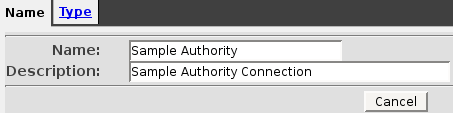
\includegraphics[width=300pt]{Generic-edit-authority-tab1}

This is the first tab of the tabbed interface you will use to edit
authority connections. The next tab is as follows:

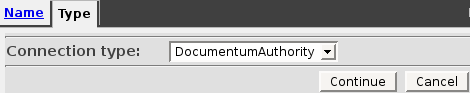
\includegraphics[width=300pt]{Generic-edit-authority-tab2}

% Licensed to the Apache Software Foundation (ASF) under one or more
% contributor license agreements. See the NOTICE file distributed with
% this work for additional information regarding copyright ownership.
% The ASF licenses this file to You under the Apache License, Version 2.0
% (the ``License''); you may not use this file except in compliance with
% the License. You may obtain a copy of the License at
%
% http://www.apache.org/licenses/LICENSE-2.0
%
% Unless required by applicable law or agreed to in writing, software
% distributed under the License is distributed on an ``AS IS'' BASIS,
% WITHOUT WARRANTIES OR CONDITIONS OF ANY KIND, either express or implied.
% See the License for the specific language governing permissions and
% limitations under the License.

\begin{picture}(1,1)
  \put(-100,15){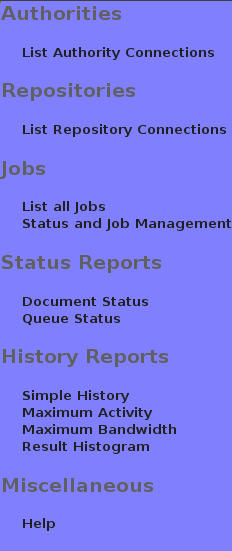
\includegraphics[width=80pt]{crawler-sidebar}}
\end{picture}


In the first two tabs you must provide a name, description, and authority
type for your new authority connection. The name should be unique on
this appliance, as you will use it to select this connection later when
making repository connections.

\note{If this appliance will be used for Aggregated Search, the authority
name for this authority must be the same on every appliance aggregating
search results. This may require coordinating authority names with other
Connector Framework administrators at other sites. For more information
on Aggregated Search, please see the \documentref{MetaCarta Appliance
Administrator's Guide}.}

The description should explain the authority connection to you or another
administrator. The authority type is the type of authority to which you
will connect.

Once you have filled in those tabs, click ``Continue'' to move on to
repository-specific options.

% Licensed to the Apache Software Foundation (ASF) under one or more
% contributor license agreements. See the NOTICE file distributed with
% this work for additional information regarding copyright ownership.
% The ASF licenses this file to You under the Apache License, Version 2.0
% (the ``License''); you may not use this file except in compliance with
% the License. You may obtain a copy of the License at
%
% http://www.apache.org/licenses/LICENSE-2.0
%
% Unless required by applicable law or agreed to in writing, software
% distributed under the License is distributed on an ``AS IS'' BASIS,
% WITHOUT WARRANTIES OR CONDITIONS OF ANY KIND, either express or implied.
% See the License for the specific language governing permissions and
% limitations under the License.

\subsubsection{Configuring a Documentum Authority Connection}

The following options apply specifically to a Documentum authority
connector.  A Documentum authority connector manages document security
to a repository in conjunction with the Documentum server (or
``docbroker'') specified in the GTS appliance configuration.  Each
Documentum authority connector connects to only one Documentum
repository (or ``docbase''). If the docbroker used by the GTS
appliance has access to more than one docbase, you will need to create
an authority connector for each repository you wish to crawl.

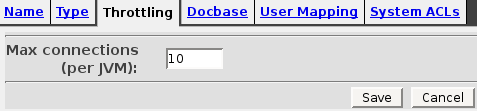
\includegraphics[width=300pt]{Docu-edit-authority-tab3}

\begin{itemize}

\item \textbf{Max Connections (per JVM):} The maximum number of
connections per JVM is important for two reasons.
\ifCombinedConnectorGuide \label{max-auth}\fi First, the number of
connections may impact the licensing on your document server,
depending on the repository. If you have a finite number of Documentum
connections available, they will be split between the authority
connector, which authorizes user access to documents, and the
repository connector, which actually downloads the documents to the
appliance. A default Documentum installation will have 100 connections
available; your Documentum installation may have more or less. It may
be advisable to lower the number of connections available to the
authority connector from the default value of 10. Ask your Documentum
administrator how many connections are available for use on your
Documentum system.

Second, the number of connections may impact the resources available
on the appliance. If the connector framework is slowing down your
appliance, lowering this number should help.

\end{itemize}

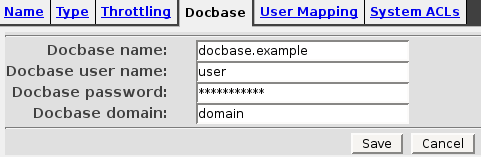
\includegraphics[width=300pt]{Docu-edit-authority-tab4}

\begin{itemize}

\item \textbf{Docbase name:} The host name of the Documentum
repository (or ``docbase'') with which you wish to connect.

\item \textbf{Docbase user name:} The user name that the GTS appliance
will use to connect to the docbase for this authority connection.
Typically, your Documentum administrator will create this account
specifically for use by the appliance. The account used by the GTS
appliance must have sufficient authority to retrieve user and group
ACLs.

\item \textbf{Docbase password:} The password corresponding to the
username given to the GTS.

\item \textbf{Docbase domain:} The domain that the docbase is part of,
typically an Active Directory domain. This is an optional argument.

\end{itemize}

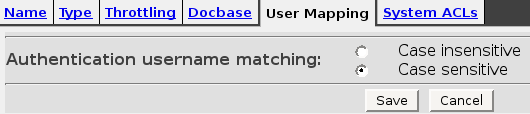
\includegraphics[width=300pt]{Docu-edit-authority-tab5}

\begin{itemize}

\item \textbf{Authentication username matching:} This option sets case
sensitivity for usernames.

\end{itemize}


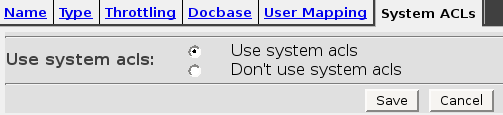
\includegraphics[width=300pt]{Docu-edit-authority-tab6}

\begin{itemize}

\item \textbf{Use system acls:} This option sets whether the GTS
appliance will use system-defined ACLs. The Documentum system
automatically generates an ACL for every folder in a docbase. Often,
ACLs of this kind are not assigned to users or groups. If your
Documentum security configuration does not use these automatically
generated ACLs, you should disable this option. The GTS appliance will
then only consider user-defined ACLs when determining file
permissions, increasing performance.

\end{itemize}




After entering this information, you will be taken to the authority
connection status page for this authority:

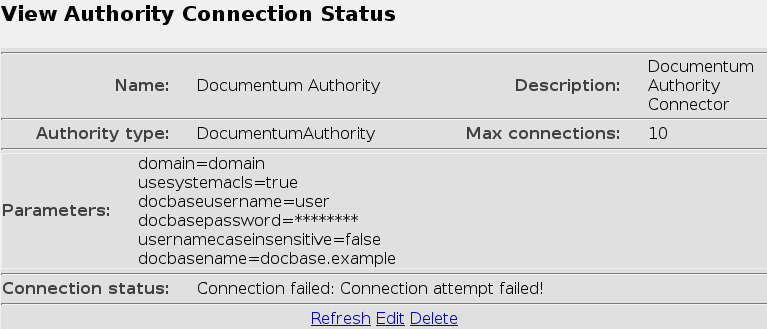
\includegraphics[width=300pt]{Docu-view-auth-conn-status}

In this example (which does not contain accurate information for any
Documentum server), the Connection Status is ``Connection failed.''
If you see this message, you most likely have incorrectly entered one
of the fields, and should click ``Edit'' to fix the data. If you have
entered everything as you intended, please inform your Documentum
administrator; you may not have been given the correct information.


% Licensed to the Apache Software Foundation (ASF) under one or more
% contributor license agreements. See the NOTICE file distributed with
% this work for additional information regarding copyright ownership.
% The ASF licenses this file to You under the Apache License, Version 2.0
% (the ``License''); you may not use this file except in compliance with
% the License. You may obtain a copy of the License at
%
% http://www.apache.org/licenses/LICENSE-2.0
%
% Unless required by applicable law or agreed to in writing, software
% distributed under the License is distributed on an ``AS IS'' BASIS,
% WITHOUT WARRANTIES OR CONDITIONS OF ANY KIND, either express or implied.
% See the License for the specific language governing permissions and
% limitations under the License.

\subsubsection{Configuring a Livelink Authority Connection}

The following options are specific to Livelink:

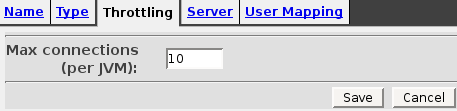
\includegraphics[width=300pt]{edit-authority-tab3}

\begin{itemize} 

\item \textbf{Max Connections (per JVM):} Here you can specify a
maximum number of connections for your authority
connection. \ifCombinedConnectorGuide The maximum number of
connections can affect system licensing and performance. See the Max
Connections item on page \pageref{max-auth} for more details.\fi

\ifLivelinkGuide
The maximum number of connections per JVM is important for two reasons.
First, the number of connections may impact the licensing on your document
server, depending on the repository. If you have a finite number of
Livelink connections available, they will be split between the authority
connector, which authorizes user access to documents, and the repository
connector, which actually downloads the documents to the appliance.

Second, the number of connections may impact the resources
available on the appliance. If the connector framework is slowing down
your appliance, lowering this number should help.
\fi

\end{itemize}

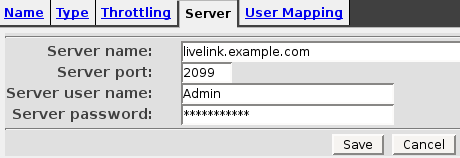
\includegraphics[width=300pt]{edit-authority-tab4}

\begin{itemize}

\item \textbf{Server name:} The name of the Livelink server from which
you wish to get authorization information.

\item \textbf{Server port:} The port on the Livelink server to which you
should connect. If you don't know what value this should be, ask your
Livelink administrator.

\item \textbf{Server user name:} The username you were given by your
Livelink administrator for connecting to the server. (The user account
must have sufficient authority to retrieve file ACLs.)

\item \textbf{Server password:} The password you were given by your
Livelink administrator for the above username.

\end{itemize}

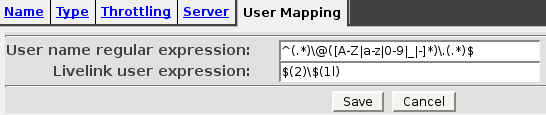
\includegraphics[width=300pt]{edit-authority-tab5}

\begin{itemize}

\label{regex}
\item \textbf{User name regular expression:} In many cases, the username
that an end-user will authenticate to GTS with is not the same as the
username that the Livelink server expects. This regular expression is used
to break the incoming username into pieces that can then be processed by
the next regular expression to produce a proper Livelink user name. The
default regular expression, \\ \verb+(.*)\@([A-Z|a-z|0-9|_|-]*)\.(.*)+,
separates an Active Directory \\ username of the form USER@DOMAIN.COM
into three distinct portions: USER, DOMAIN, and COM. In many cases,
this expression will be sufficient for you.

\note{If you are not familiar with regular expressions, there
are a variety of tutorials available on the web, including
\url{http://gnosis.cx/publish/programming/regular_expressions.html}
and \url{http://perldoc.perl.org/perlrequick.html}. If you still have
difficulty with these settings, please contact Customer Support (see
page \pageref{SupportContact}).}

\item \textbf{Livelink user expression:} Once you have deconstructed
the Active Directory username, you need to put it back together as an
appropriate Livelink username for your site's Livelink instance. The
default is the expression \verb+$(2)\$(1l)+, which takes the second value
from the first regular expression (DOMAIN), adds a backslash
(\verb+\+), and then puts the first value from the first expression in
place in lowercase (user), producing \verb+DOMAIN\user+. Depending on
how your Livelink instance is configured, you may need to change this
value. 

This expression may contain either plain text or variable expressions
such as \verb+$(2)+ above.  A variable expression, which must be of
the form \verb+$(N)+ where N is a number, represents a string from the
regular expression defined previously. You can force the string to be
all uppercase or lowercase by appending a \verb+u+ or \verb+l+ to the
string number. For example, to make the third string all in uppercase,
you would use \verb+$(3u)+. A dollar sign character must be escaped
with another dollar sign before it, so \verb+$$+ in this text box will
produce \verb+$+ in the user expression.

\end{itemize}

After entering this information, you will be taken to the authority
connection status page for this authority:

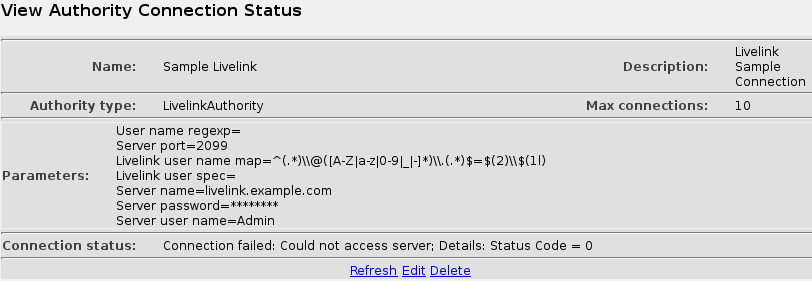
\includegraphics[width=300pt]{view-auth-conn-status}

In this example (which does not contain accurate information for any
Livelink server), the Connection Status is ``Connection failed.''
If you see this message, you most likely have incorrectly entered one
of the fields, and should click ``Edit'' to fix the data. If you have
entered everything as you intended, please inform your Livelink administrator;
you may not have been given the correct information.



\subsection{Creating Repository Connections}

Once you have created an authority connection, you need to create a
repository connection.
To do so, click ``List Repository Connections'' on the sidebar menu. Then,
when presented with the list of repository connections, click ``Add a
new connection.'' You will see the following two tabs:

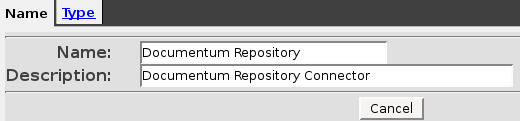
\includegraphics[width=300pt]{Docu-edit-repository-tab1}

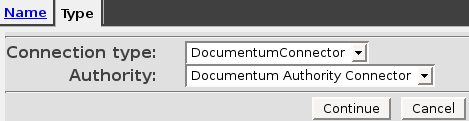
\includegraphics[width=300pt]{Docu-edit-repository-tab2}

Now you must provide a name, description, connector type, and authority
type for your new repository connection. The name should be unique,
as you will use it to select this connection later when defining
jobs. The description should explain the repository connection to you
or another administrator.  The connector type is the type of repository
from which you will get documents. The authority type is the type of
authority from which you will get authorization information. In the case
of a Documentum Connector or Livelink Connector, you may have set up an
authority connection. If you select that authority connection here, the
permissions associated with the ingested documents will be the same as the
permissions of the original documents in the repository. If you intend
to force AD ACLs on your documents or are setting up a JDBC Connector,
RSS Connector, or Share Connector, then you should select ``Standard
(Kerberos)'' here.

Once you have filled in those tabs and click continue to move on to
the repository-specific options.

% Licensed to the Apache Software Foundation (ASF) under one or more
% contributor license agreements. See the NOTICE file distributed with
% this work for additional information regarding copyright ownership.
% The ASF licenses this file to You under the Apache License, Version 2.0
% (the ``License''); you may not use this file except in compliance with
% the License. You may obtain a copy of the License at
%
% http://www.apache.org/licenses/LICENSE-2.0
%
% Unless required by applicable law or agreed to in writing, software
% distributed under the License is distributed on an ``AS IS'' BASIS,
% WITHOUT WARRANTIES OR CONDITIONS OF ANY KIND, either express or implied.
% See the License for the specific language governing permissions and
% limitations under the License.

\subsubsection{Configuring a Documentum Repository}

You must fill in the following extra fields if you choose to
configure a Documentum repository connection: 

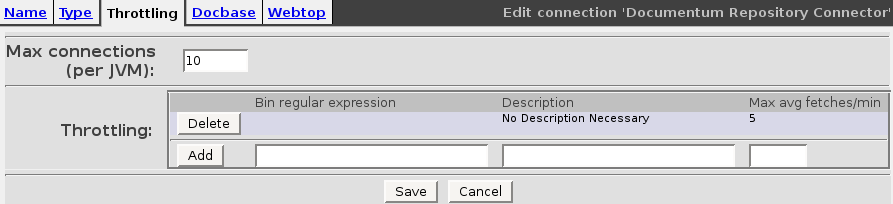
\includegraphics[width=300pt]{Docu-edit-repository-tab3}


\begin{itemize}

\item \textbf{Max connections (per JVM):} \ifCombinedConnectorGuide \label{maxrepocon} \fi Here you can set the maximum
number of connections to your repository.

The maximum number of connections per JVM is important for three
reasons.  First, the number of connections may impact the licensing on
your document server, depending on the repository. If you have a
finite number of Documentum connections available, they will be split
between the authority connector, which authorizes user access to
documents, and the repository connector, which actually downloads the
documents to the appliance. As in the case of the authority
connection, the default value of 10 connections may be a larger
portion of the available connections than you would like the GTS
appliance to use.

Second, the number of connections may impact the resources
available on the appliance. If the connector framework is slowing down
your appliance, lowering this number should help.

Third, only ten document streams can be processed by the appliance at
one time.  If you are also using other repository connectors or the
\command{ingest} command on the appliance, you should reduce this
number to prevent contention for the Ingestion interface. The
Documentum Connector will never overwhelm the interface on its own,
but when other applications are also using the ingestion interface, it
may be best to set the number of repository connections to five or
even fewer.

\item \textbf{Throttling:} Throttling allows you to limit the rate of
document ingestion based on document bins that you create with regular
expressions.

The maximum fetch rate allows you to set three things: Expression,
description, and fetches per minute. Expression allows you to provide
a regular expression to match against document bins. Each document
ingested through a connector is associated with one or more document
bins. These bins represent the servers that the connector interacts
with to obtain the document. Typically, a document will be associated
with only one document bin, representing the repository server hosting
the document. For some repository connections, documents ingested
through the connector can be hosted by different servers. In the
Documentum Connector, documents can only come from one docbase, which
you will set on the following tab. Simply leave the expression blank;
this will match any docbase you enter on the following tab.  All you
need to set is the number of document fetches per minute.  Description
is an optional field that allows you to provide a short text
description of the throttle.  Once you have set the fetch rate and
optional description, click Add.

\end{itemize}

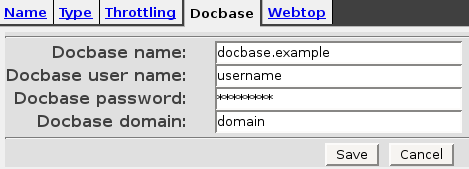
\includegraphics[width=300pt]{Docu-edit-repository-tab4}

\begin{itemize}

\item \textbf{Docbase name:} The host name of the Documentum
repository (or ``docbase'') with which you wish to connect.

\item \textbf{Docbase user name:} The user name that the GTS appliance
will use to connect to the docbase for this repository connection.
Typically, your Documentum administrator will create this account
specifically for use by the appliance. The account used by the GTS
appliance must have sufficient authority to retrieve files and their
corresponding ACLs. This may or may not be the same account used by
the GTS appliance for authority connections, depending on the security
model enforced by your Documentum administrator.

\item \textbf{Docbase password:} The password corresponding to the
username given to the GTS.

\item \textbf{Docbase domain:} The domain that the docbase is part of,
typically an Active Directory domain. This is an optional argument.

\end{itemize}

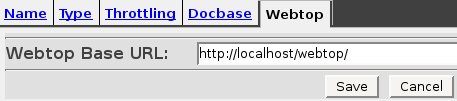
\includegraphics[width=300pt]{Docu-edit-repository-tab5}

\begin{itemize}

\item \textbf{Webtop Base URL:} The URL of the Webtop server that the
GTS appliance will use to provide MetaCarta Web Search Interface users
with document links in search results. It is recommended that you
select a Webtop server that connects to the same docbroker that the
GTS appliance uses.

\end{itemize}

After entering this information, you will be taken to the status page
for this repository connection:

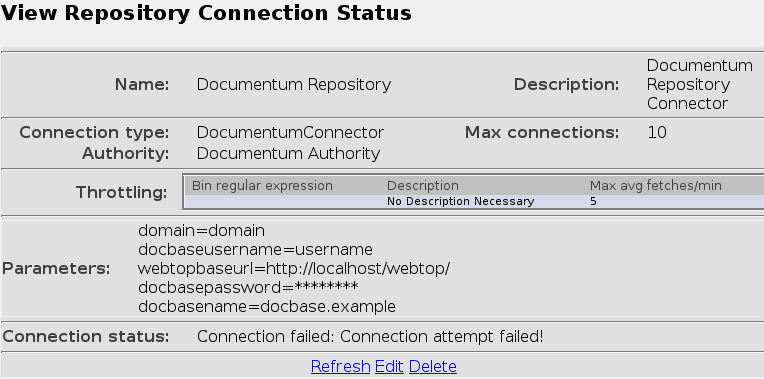
\includegraphics[width=300pt]{Docu-view-repo-conn-status}

In this example (which does not contain accurate information for any
Documentum server), the Connection Status is ``Connection failed.''
If you see this message, you most likely have incorrectly entered one
of the fields, and should click ``Edit'' to fix the data. If you have
entered everything as you intended, please inform your Documentum
administrator; you may not have been given the correct information.



% Licensed to the Apache Software Foundation (ASF) under one or more
% contributor license agreements. See the NOTICE file distributed with
% this work for additional information regarding copyright ownership.
% The ASF licenses this file to You under the Apache License, Version 2.0
% (the ``License''); you may not use this file except in compliance with
% the License. You may obtain a copy of the License at
%
% http://www.apache.org/licenses/LICENSE-2.0
%
% Unless required by applicable law or agreed to in writing, software
% distributed under the License is distributed on an ``AS IS'' BASIS,
% WITHOUT WARRANTIES OR CONDITIONS OF ANY KIND, either express or implied.
% See the License for the specific language governing permissions and
% limitations under the License.

\subsubsection{Configuring a JDBC Connector}

You must fill in the following tabs if you are configuring a JDBC
Connector:

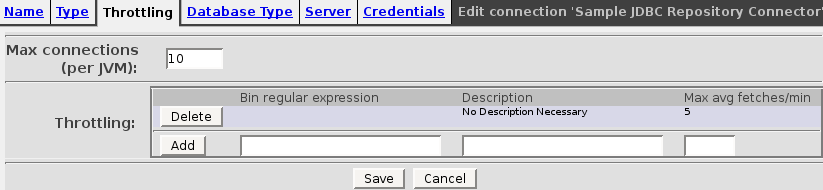
\includegraphics[width=300pt]{JDBC-edit-repository-tab3}

\begin{itemize}

\item \textbf{Max connections (per JVM):} Here you can set the maximum
number of connections to your repository.  \ifCombinedConnectorGuide
The maximum number of connections per JVM is important for three
reasons; licensing, appliance resources, and the possiblity of
overwhelming the ingestion interface. For a more complete explanation,
see the Max Connections item on page \pageref{maxrepocon}.\fi

\ifJDBCGuide
The maximum number of connections per JVM is important for three reasons.
First, the number of connections may impact the licensing on your document
server, depending on the repository.

Second, the number of connections may impact the resources
available on the appliance. If the connector framework is slowing down
your appliance, lowering this number should help.

Third, only ten document streams can be processed by the appliance
at one time.  If you are also using other repository connectors or
the \command{ingest} command on the appliance, you should reduce this
number to prevent contention for the Ingestion interface. The JDBC
Connector will never overwhelm the interface on its own, but when other
applications are also using the ingestion interface, it may be best to
set the number of repository connections to five or even fewer.
\fi


\item \textbf{Throttling:} Here you can set a maximum document fetch
rate for the repository connection.

The maximum fetch rate allows you to set three things: Expression,
description, and fetches per minute. Expression allows you to provide
a regular expression to match against document bins.  Each document
ingested through a connector is associated with one or more document
bins. These bins represent the servers that the connector interacts
with to obtain the document.  Typically, a document will be associated
with only one document bin, representing the repository server hosting
the document. For some repository connections, documents ingested
through the connector can be hosted by different servers. In the JDBC
Connector, documents only come from one server, which you will set on
the ``Server'' tab. Simply leave the expression blank; this will match
any server you enter on the ``Server'' tab.  All you need to set is
the number of document fetches per minute.  Description is an optional
field that allows you to provide a short text description of the
throttle.  Once you have set the fetch rate and optional description,
click Add.


\end{itemize}

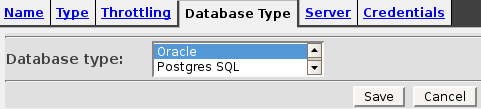
\includegraphics[width=300pt]{JDBC-edit-repository-tab4}

\begin{itemize}

\item \textbf{Database Type:} Here you should select the type of
database to which you are connecting. Currently supported databases
include Oracle, Postgres SQL, MS SQL Server (Version greater than
6.5), and Sybase (Version 10 and greater).

\end{itemize}

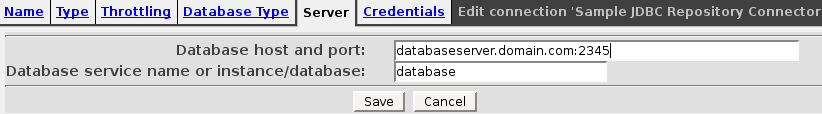
\includegraphics[width=300pt]{JDBC-edit-repository-tab5}

\begin{itemize}

\item \textbf{Server Database Host and Port:} Ask your database
administrator to provide you with the correct host name and port
number for your repository. This should be of the form
\url{databaseserver.domain.com:port}.

\item \textbf{Database service name or instance/database:} This should
be the name of the database you wish to crawl in the form
\command{database} or \linebreak \command{instance/database}.

\end{itemize}

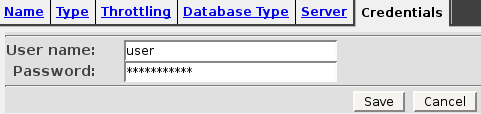
\includegraphics[width=300pt]{JDBC-edit-repository-tab6}

\begin{itemize}

\item \textbf{Name:} This is the username that the GTS appliance will
use to connect to your database server. It is recommended that the GTS
appliance be given its own username in the system. The appliance will
need to be granted appropriate permissions to select from the tables
you wish to crawl.

\item \textbf{Password:} This is the password that corresponds to the
username provided above.

\end{itemize}


After entering this information, you will be taken to the repository 
connection status page for this repository:

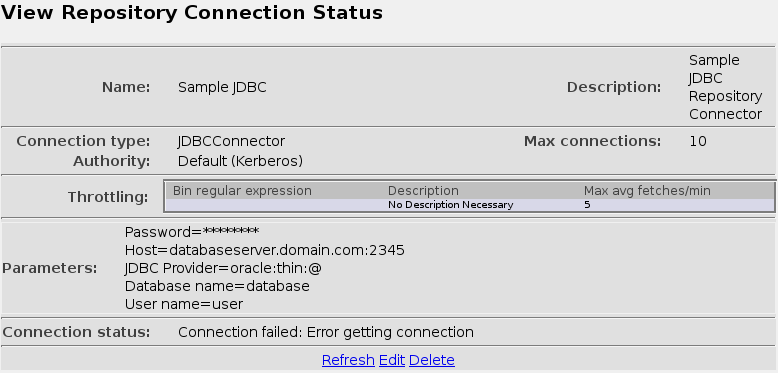
\includegraphics[width=300pt]{JDBC-view-repo-conn-status}

In this example (which does not contain accurate information for any
JDBC Connector), the Connection Status is ``Connection failed.''
If you see this message, you most likely have incorrectly entered one
of the fields, and should click ``Edit'' to fix the data. If you have
entered everything as you intended, please inform your database administrator;
you may not have been given the correct information.


% Licensed to the Apache Software Foundation (ASF) under one or more
% contributor license agreements. See the NOTICE file distributed with
% this work for additional information regarding copyright ownership.
% The ASF licenses this file to You under the Apache License, Version 2.0
% (the ``License''); you may not use this file except in compliance with
% the License. You may obtain a copy of the License at
%
% http://www.apache.org/licenses/LICENSE-2.0
%
% Unless required by applicable law or agreed to in writing, software
% distributed under the License is distributed on an ``AS IS'' BASIS,
% WITHOUT WARRANTIES OR CONDITIONS OF ANY KIND, either express or implied.
% See the License for the specific language governing permissions and
% limitations under the License.

\subsubsection{Configuring a Livelink Repository}

You must fill in the following extra tabs if you are creating a
Livelink repository connection:

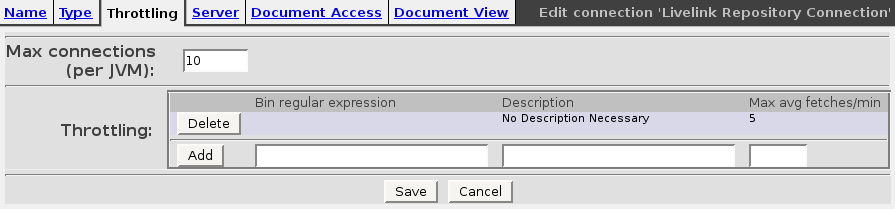
\includegraphics[width=300pt]{edit-repository-tab3}

\begin{itemize}

\item \textbf{Max connections (per JVM):} Here you can specify a
maximum number of connections for your repository. \ifCombinedConnectorGuide
The maximum number of connections per JVM is important for three
reasons; licensing, appliance resources, and the possiblity of
overwhelming the ingestion interface. For a more complete explanation,
see the Max Connections item on page \pageref{maxrepocon}.\fi

\ifLivelinkGuide
The maximum number of connections per JVM is important for three reasons.
First, the number of connections may impact the licensing on your document
server, depending on the repository. If you have a finite number of
Livelink connections available, they will be split between the authority
connector, which authorizes user access to documents, and the repository
connector, which actually downloads the documents to the appliance.

Second, the number of connections may impact the resources
available on the appliance. If the connector framework is slowing down
your appliance, lowering this number should help.

Third, only ten document streams can be processed by the appliance
at one time.  If you are also using other repository connectors or
the \command{ingest} command on the appliance, you should reduce this
number to prevent contention for the Ingestion interface. The Livelink
Connector will never overwhelm the interface on its own, but when other
applications are also using the ingestion interface, it may be best to
set the number of repository connections to five or even fewer.
\fi

\item \textbf{Throttling:} This allows you to set a maximum document
fetch rate from the repository.


The maximum fetch rate allows you to set three things: Expression,
description, and fetches per minute. Expression allows you to provide
a regular expression to match against document bins.  Each document
ingested through a connector is associated with one or more document
bins. These bins represent the servers that the connector interacts
with to obtain the document.  Typically, a document will be associated
with only one document bin, representing the repository server hosting
the document. For some repository connections, documents ingested
through the connector can be hosted by different servers. In the
Livelink Connector, documents only come from one server, which you
will set on the following tab. Simply leave the expression blank; this
will match any server you enter on the following tab.  All you need to
set is the number of document fetches per minute.  Description is an
optional field that allows you to provide a short text description of
the throttle.  Once you have set the fetch rate and optional
description, click Add.


\end{itemize}

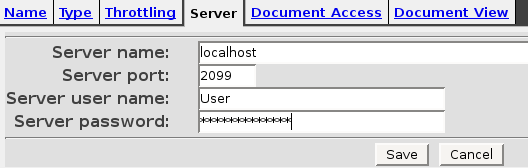
\includegraphics[width=300pt]{edit-repository-tab4}

\begin{itemize}

\item \textbf{Server name:} The name of the Livelink server from which you wish
to crawl documents.

\item \textbf{Server port:} The port on the Livelink server to which you
should connect. If you don't know what value this should be, ask your
Livelink administrator.

\item \textbf{Server user name:} The username you were given by your
Livelink administrator for connecting to the server. (The user account
must have sufficient authority to retrieve documents.)

\item \textbf{Server password:} The password you were given by your
Livelink administrator for the above username.

\end{itemize}

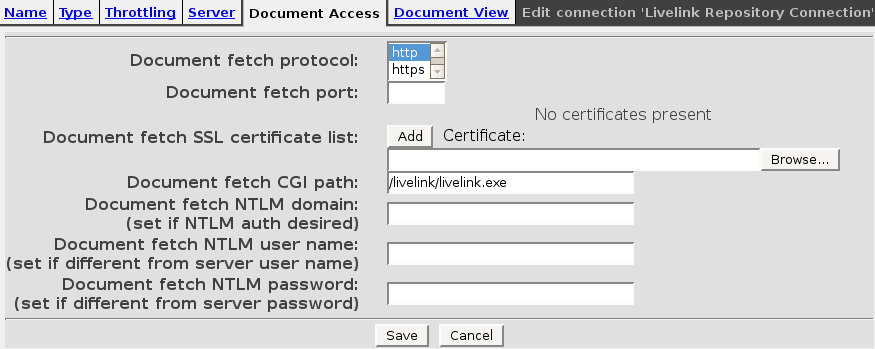
\includegraphics[width=300pt]{edit-repository-tab5}

These options all concern ``fetching'' documents, that is, the paths
that the Connector Framework should use when collecting documents for
ingestion to the MetaCarta search system. 

\begin{itemize}

\item \textbf{Document fetch protocol:} If you are connecting to an
open Livelink repository, choose ``http.'' If you are connecting using
SSL, choose ``https.''

\item \textbf{Document fetch port:} The port to use when connecting
to the Livelink server. If you are using the default port (80 for
http, 443 for https) you can leave this field blank. 

\item \textbf{Document fetch SSL certificate list:} Some Livelink servers
require that you authenticate via SSL before downloading documents. By
clicking the ``Browse'' button, you can select an SSL certificate that
the appliance should trust for authentication to the Livelink server. Clicking
``Add'' will upload the certificate to the appliance.

To get such a certificate, visit the Livelink repository from your
web browser and save the file, or ask your Livelink administrator.
For maximum robustness, you should add the certificate for the certificate
authority that signed the Livelink repository certificate rather than
the Livelink certificate itself. To do this, contact your site's security
administrators. In some cases, you may need more than one certificate.

\item \textbf{Document fetch CGI path:} The path on the Livelink server that the
appliance should use to crawl for documents.

\item \textbf{Document fetch NTLM domain:} The NTLM domain 
through which the crawler should access the Livelink repository, if required.

\item \textbf{Document fetch NTLM user name:} The user name to use for 
NTLM, if different from the user name used to connect to the server.

\item \textbf{Document fetch NTLM password:} The password to use for
NTLM, if different from the password used to connect to the server.

\end{itemize}

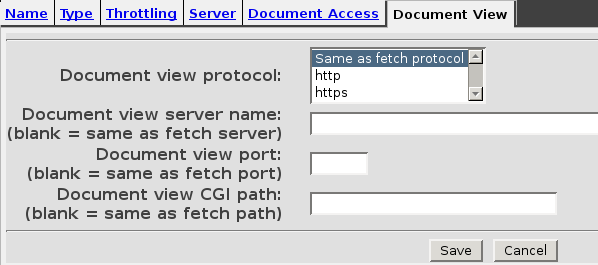
\includegraphics[width=300pt]{edit-repository-tab6}

These options all concern ``viewing'' documents, that is, the URLs
at which users are directed to documents when they see the documents
as search results. These options can be used to change the URLs of
documents crawled through Livelink before they are sent to the MetaCarta
Ingestion API. They do not change anything about the documents in the
Livelink repository itself. 

\begin{itemize}

\item \textbf{Document view protocol:} If end users are connecting to an open
Livelink repository, choose ``http.'' If users are connecting using SSL,
choose ``https.'' If users are connecting to the same Livelink instance
as the crawler, choose ``Same as fetch protocol.''

\item \textbf{Document view server:} The server to use when giving end
users links to a Livelink server as part of search results. If you
are using the same server as for document fetch, you can leave this
field blank.

\item \textbf{Document view port:} The port to use when giving end users
links to the Livelink server as part of search results. If you are using
the same port as for document fetch, you can leave this field blank.

\item \textbf{Document view CGI path:} The path on the Livelink server
that the end user should use when viewing document search results. This
is usually the same as the fetch path, but if it is not, you can set
it here. If this is different from the document fetch CGI path, it is
likely because the appliance has different permissions from normal users,
but it may also be because you want users to access a different Livelink
server from the appliance. This setting (along with the NTLM domain,
described above) determines the URL given to users of the Web Search
Interface, MetaCarta Search APIs, and the ESRI ArcMap Extension.

\end{itemize}


After entering this information, you will be taken to the repository 
connection status page for this repository:

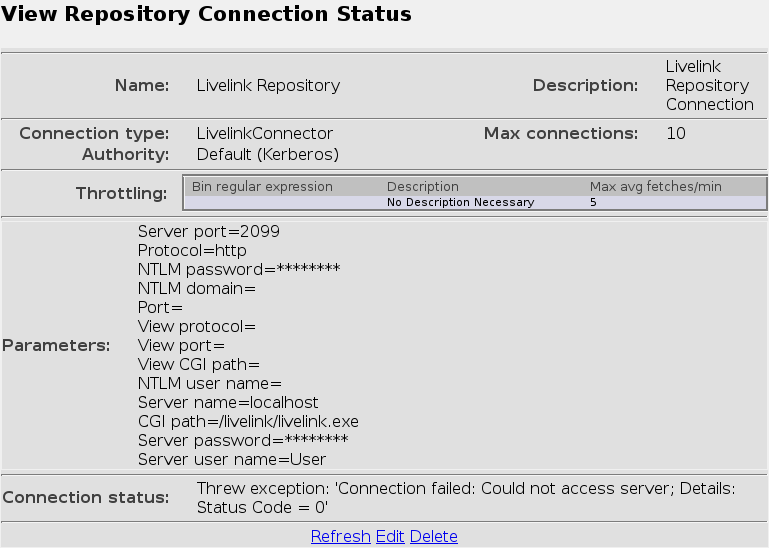
\includegraphics[width=300pt]{view-repo-conn-status}

In this example (which does not contain accurate information for any
Livelink server), the Connection Status is ``Connection failed.''
If you see this message, you most likely have incorrectly entered one
of the fields, and should click ``Edit'' to fix the data. If you have
entered everything as you intended, please inform your Livelink administrator;
you may not have been given the correct information.


% Licensed to the Apache Software Foundation (ASF) under one or more
% contributor license agreements. See the NOTICE file distributed with
% this work for additional information regarding copyright ownership.
% The ASF licenses this file to You under the Apache License, Version 2.0
% (the ``License''); you may not use this file except in compliance with
% the License. You may obtain a copy of the License at
%
% http://www.apache.org/licenses/LICENSE-2.0
%
% Unless required by applicable law or agreed to in writing, software
% distributed under the License is distributed on an ``AS IS'' BASIS,
% WITHOUT WARRANTIES OR CONDITIONS OF ANY KIND, either express or implied.
% See the License for the specific language governing permissions and
% limitations under the License.

\subsubsection{Configuring a Share Connection}

You must fill in the following tabs if you are configuring a Share
connection:

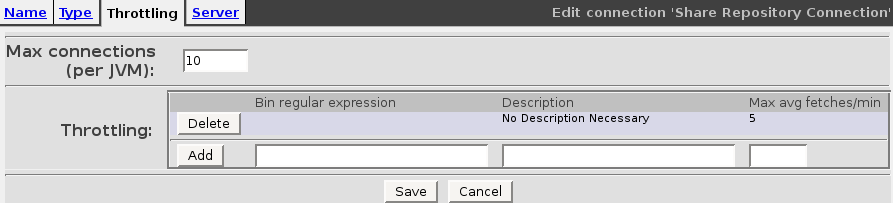
\includegraphics[width=300pt]{Share-edit-repository-tab3}

\begin{itemize}

\item \textbf{Max connections (per JVM):} Here you can set the maximum
number of connections to your repository.  \ifCombinedConnectorGuide
The maximum number of connections per JVM is important for three
reasons; licensing, appliance resources, and the possiblity of
overwhelming the ingestion interface. For a more complete explanation,
see the Max Connections item on page \pageref{maxrepocon}.\fi

\ifShareGuide
The maximum number of connections per JVM is important for three reasons.
First, the number of connections may impact the licensing on your document
server, depending on the repository.

Second, the number of connections may impact the resources
available on the appliance. If the connector framework is slowing down
your appliance, lowering this number should help.

Third, only ten document streams can be processed by the appliance
at one time.  If you are also using other repository connectors or
the \command{ingest} command on the appliance, you should reduce this
number to prevent contention for the Ingestion interface. The Share
Connector will never overwhelm the interface on its own, but when other
applications are also using the ingestion interface, it may be best to
set the number of repository connections to five or even fewer.
\fi

\item \textbf{Throttling:} Here you can set a maximum document fetch
rate for the repository connection.


The maximum fetch rate allows you to set three things: Expression,
description, and fetches per minute. Expression allows you to provide
a regular expression to match against document bins.  Each document
ingested through a connector is associated with one or more document
bins. These bins represent the servers that the connector interacts
with to obtain the document.  Typically, a document will be associated
with only one document bin, representing the repository server hosting
the document. For some repository connections, documents ingested
through the connector can be hosted by different servers. In the Share
Connector, documents only come from one server, which you will set on
the following tab. Simply leave the expression blank; this will match
any server you enter on the following tab.  All you need to set is the
number of document fetches per minute.  Description is an optional
field that allows you to provide a short text description of the
throttle.  Once you have set the fetch rate and optional description,
click Add.




\end{itemize}

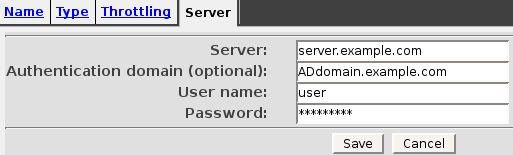
\includegraphics[width=300pt]{Share-edit-repository-tab4}

\begin{itemize}

\item \textbf{Server:} The fully qualified sever name of network share
with which you wish to connect.

\item \textbf{Authentication domain (optional):} The Active Directory
domain that your network share is a part of. This is an optional
argument. 

\item \textbf{User name:} The user name that the GTS appliance will
use to connect to the network share for this repository connection.
Typically, your network share administrator will create this account
specifically for use by the appliance. The account used by the GTS
appliance must have sufficient authority to retrieve files and their
corresponding ACLs.

\item \textbf{Password:} The password corresponding to the
user name given to the GTS.

The Active Directory domain should only be included once between the
``Authentication domain'' and ``User name'' fields, but may not be
necessary for either. The exact phrasing required by the crawler
depends on the configuration of your network share. This is a common
cause of a failed repository connection. In order to correctly
configure your repository connection you may need to try all 3
possible pairings: \command{ADdomain.example.com} with \command{user}, a
blank domain with \command{user@ADdomain.example.com}, and a blank
domain with \command{user}.

\end{itemize}

\note{The Share Connector gets its domain authentication information by
querying the relevant AD domain for a list of domain controllers and
then trying the first domain controller on that list. If your domain
controllers are inaccessible, the Share Connector will not be able to
function.} 

% This should go in a Troubleshooting section when we have one,
% but rc4 is not the time.

After entering this information, you will be taken to the repository 
connection status page for this repository:

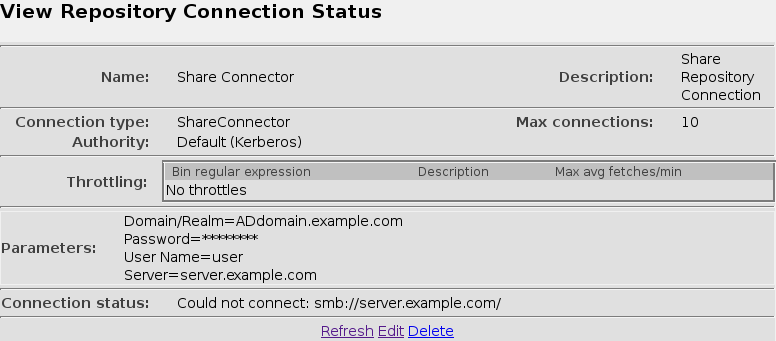
\includegraphics[width=300pt]{Share-view-repo-conn-status}

In this example (which does not contain accurate information for any
Share Connector), the Connection Status is ``Connection failed.''  If
you see this message, you most likely have incorrectly entered one of
the fields, and should click ``Edit'' to fix the data. If you have
entered everything as you intended, please inform your network share
administrator; you may not have been given the correct information.


% Licensed to the Apache Software Foundation (ASF) under one or more
% contributor license agreements. See the NOTICE file distributed with
% this work for additional information regarding copyright ownership.
% The ASF licenses this file to You under the Apache License, Version 2.0
% (the ``License''); you may not use this file except in compliance with
% the License. You may obtain a copy of the License at
%
% http://www.apache.org/licenses/LICENSE-2.0
%
% Unless required by applicable law or agreed to in writing, software
% distributed under the License is distributed on an ``AS IS'' BASIS,
% WITHOUT WARRANTIES OR CONDITIONS OF ANY KIND, either express or implied.
% See the License for the specific language governing permissions and
% limitations under the License.

\subsubsection{Configuring an RSS Connector}

You must fill in the following tabs if you are configuring an RSS
Connector:

\bigimage{RSS-edit-repository-tab3}

\begin{itemize}

\item \textbf{Max connections (per JVM):} Here you can set the maximum
number of connections to your repository.  \ifCombinedConnectorGuide
The maximum number of connections per JVM is important for three
reasons; licensing, appliance resources, and the possiblity of
overwhelming the ingestion interface. For a more complete explanation,
see the Max Connections item on page \pageref{maxrepocon}.\fi

\ifJDBCGuide
The maximum number of connections per JVM is important for two reasons.
First, the number of connections may impact the resources
available on the appliance. If the connector framework is slowing down
your appliance, lowering this number should help.

Second, only ten document streams can be processed by the appliance
at one time.  If you are also using other repository connectors or
the \command{ingest} command on the appliance, you should reduce this
number to prevent contention for the Ingestion interface. The RSS
Connector will never overwhelm the interface on its own, but when other
applications are also using the ingestion interface, it may be best to
set the number of repository connections to five or even fewer.
\fi


\item \textbf{Throttling:} Here you can set a maximum average document fetch
rate for the repository connection. The maximum fetch rate allows you
to set three things: Expression, description, and fetches per minute.

In the RSS Connector, the value set in the expression field is a
server name. To throttle an individual server, use its name as the
expression and set the number of document fetches per minute. We
recommend a maximum average rate of 6 fetches per minute.  Once you
have set that, click Add.
\end{itemize}

In general, you should be conscientious about document fetch rates,
feed query rates, download rates, and other rates related to server
traffic when using the RSS Connector to connect to public, external
servers. The recommended rates suggested in this guide are typically
an upper limit. You should not exceed these suggestions for external
servers. Higher demands on these servers may produce undesirable
effects in their performance; the administrators of those servers may
block your connection.

If your organization uses RSS publishing internally, you should speak
to your server administrators about appropriate rate limits.

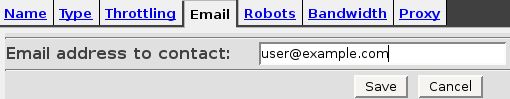
\includegraphics[width=300pt]{RSS-edit-repository-tab4}

\begin{itemize}

\item \textbf{Email:} A contact email address. This email address is included in request headers sent to servers. Administrators of servers recieving these requests may wish to contact you regarding your interactions with their content servers.

\end{itemize}

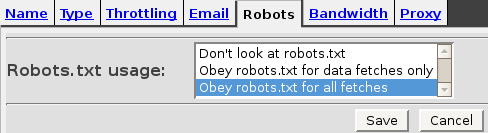
\includegraphics[width=300pt]{RSS-edit-repository-tab5}

\begin{itemize}

\item \textbf{Robots.txt Usage:} This determines whether the crawler obeys guidelines from the \dirpath{robots.txt} file on a server. There are three options:

\begin{itemize}

\item \textbf{Don't look at robots.txt}

\item \textbf{Obey robots.txt for data fetches only}

\item \textbf{Obey robots.txt for all fetches}

\end{itemize}

By default, \textbf{Obey robots.txt for all fetches} is selected. When
selected, the crawler will obey all interfacing and downloading
guidelines set in a server's \dirpath{robots.txt} file. You should
always use this setting when connecting to servers on the open Internet.

\end{itemize}

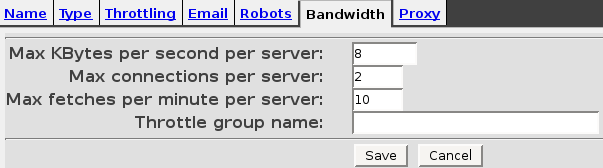
\includegraphics[width=300pt]{RSS-edit-repository-tab6}

\begin{itemize}


\item \textbf{Max KBytes per second per server:} The maximum download rate
from each server, which will include all content from that server. This
should be no more than 8 kilobytes per second for servers on the open
Internet

\item \textbf{Max connections per server:} The maximum number of
connections to each server. This should be 1 or 2 for servers on the
open Internet.

\item \textbf{Max fetches per minute per server:} The maximum number of
document fetches per minute for each server. This should be no higher
than 10 fetches per minute for servers on the open Internet.

\item \textbf{Throttle group name:} (Optional) Connections that have the
same throttle group name will be throttled together. A blank name will
match all other named groups. You should give repository connections
that will be used to crawl the same servers the same throttle group name.

\end{itemize}

If your organization uses RSS publishing internally, you should
consult your system administrator about appropriate limits.

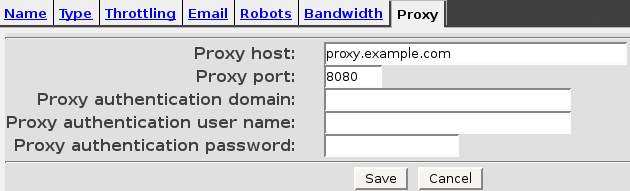
\includegraphics[width=300pt]{RSS-edit-repository-tab7}

This tab allows you to set up a proxy host if your MetaCarta appliance
needs a proxy server to forward requests outside of your
local network. If your appliance and proxy server are part of an NTLM
domain, you will need to include domain information and a user name
and password associated with that domain that has access to the proxy
server.

\begin{itemize}

\item \textbf{Proxy host:} The proxy server host name.

\item \textbf{Proxy port:} The port used to communicate with the proxy server. Often, this is port 8080. Ask the administrator of your proxy server for the port number you should enter here.

\item \textbf{Proxy authentication domain:} (Optional) The NTLM authentication domain of the proxy server and appliance.

\item \textbf{Proxy authentication user name:} (Optional) The user name given to the appliance for use in the domain. This user name should have access to the proxy server.

\item \textbf{Proxy authentication password:} (Optional) The password corresponding with that user name.

\end{itemize}


After entering this information, you will be taken to the repository
connection status page for this repository:

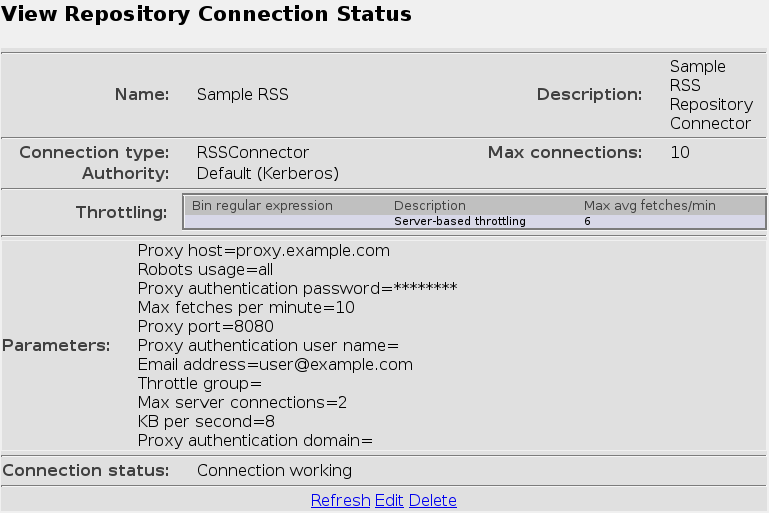
\includegraphics[width=300pt]{RSS-view-repo-conn-status}

In this example, the Connection Status is ``Connection working.''  If the
Connection Status is ``Connection failed,'' you might have have entered
some information (particularly your proxy information) incorrectly. If
so, click ``Edit'' to fix the data.


\subsection{Creating and Running Jobs}

To run a job, click ``Status and Job Management'' on the sidebar menu.
You can run or edit existing jobs from this menu.

To create a new job, click ``List All Jobs'' on the sidebar menu. Then, when
presented with the list of current jobs, click ``Add a new job.'' You
will be presented with two tabs, in which you must fill in the following
information:

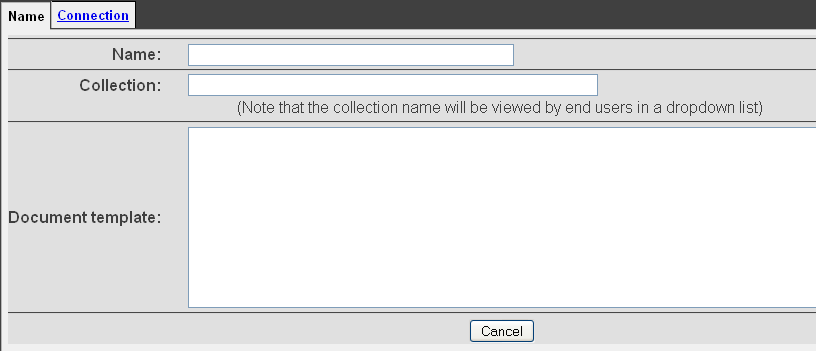
\includegraphics[width=300pt]{Generic-edit-job-tab1}

\begin{itemize}

\item \textbf{Name:} The name of the job. You will use this to identify
the job later.

\item \textbf{Collection:} The collection name metadata for all
documents in this job. Users of the MetaCarta Web Search Interface or
other search tools can use this name to select the set of documents in
this job. For more information on collection name metadata, please see
the \documentref{MetaCarta Appliance Administrator's Guide}.

\item \textbf{Document Template:} The document template with which you
would like all documents in this job ingested.  Document Templates allow
you to define what parts of a document should be indexed, what parts
should be ignored, and what date to use as the principal date of the
document. For more information, please see the \documentref{MetaCarta
Document Templates Integrator's Guide}.


\end{itemize}

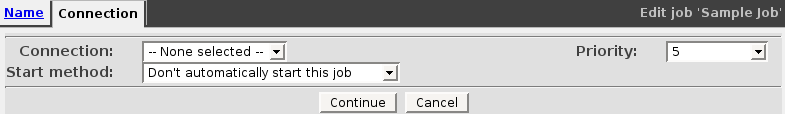
\includegraphics[width=300pt]{Generic-edit-job-tab2}

\begin{itemize}

\item \textbf{Connection:} The name of the repository connection you
wish to use for this job. You select this from the list of repository
connections you have already made. You may have more than one job use
the same repository connection, but if you have two jobs crawl the same
documents, the documents will have the metadata and collection name
associated with whatever job crawled the document most recently. This
will cause unpredictable results when searching those collections,
searching for those documents, or trying to delete those collections.
We recommend never crawling the same document in two different jobs.

\item \textbf{Start method:} When you want the job to start
automatically. The job can automatically start the next time it is
scheduled to run (``Start when schedule window starts''), or not at
all (``Don't automatically start this job''). If you select ``Start
even inside a schedule window'', the job will start whenever its
schedule window is open and it is not running. Thus, if the job
finishes during its one of its schedule windows, it will restart
immediately. If it is created during one if its schedule windows, it
will start immediately. Scheduling windows will be explained in the
``Scheduling'' section.

\item \textbf{Priority:} From 1 (highest) to 10 (lowest), the priority
this crawl should have if it must compete for resources with other
crawls on the appliance. You should not need to change this unless you
are running more than one crawl at the same time; if you are, assign a
higher priority to the crawls whose documents you want to be processed
preferentially before documents from other jobs.

\end{itemize}

After filling in those options, click ``Continue,'' and you will be
presented with additional repository-specific tabs. 

% Licensed to the Apache Software Foundation (ASF) under one or more
% contributor license agreements. See the NOTICE file distributed with
% this work for additional information regarding copyright ownership.
% The ASF licenses this file to You under the Apache License, Version 2.0
% (the ``License''); you may not use this file except in compliance with
% the License. You may obtain a copy of the License at
%
% http://www.apache.org/licenses/LICENSE-2.0
%
% Unless required by applicable law or agreed to in writing, software
% distributed under the License is distributed on an ``AS IS'' BASIS,
% WITHOUT WARRANTIES OR CONDITIONS OF ANY KIND, either express or implied.
% See the License for the specific language governing permissions and
% limitations under the License.

\subsubsection{Documentum Job Options}

You must fill in the following extra fields if you choose to
configure a Documentum repository connection: 

\bigimage{Docu-edit-job-tab3}

\input{schedule-input}

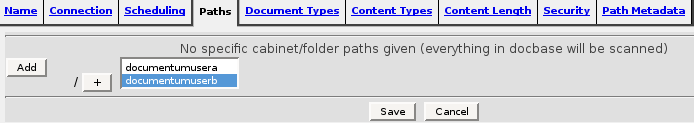
\includegraphics[width=300pt]{Docu-edit-job-tab4}

\begin{itemize}

\item \textbf{Paths:} The directory paths in your Documentum
repository from which you want your crawl to start. You can specify
one or more directory paths. If you do not specify directory paths,
the job will crawl all directories on your Documentum repository. You
can build directory paths by selecting individual directories. To
start, select the base directory of the path you wish to create, then
click the ``+'' button. A new selection box will appear with the
directories contained by that parent directory. Select a directory at
that level and click the ``+'' button. Continue building your
directory path in this fashion. When it's complete, click ``Add''. A
new selection box will appear beneath the added directory path. You
can continue to add more directory paths to your list. To remove a
directory path from the list, click the ``Delete'' button next to it.


\end{itemize}

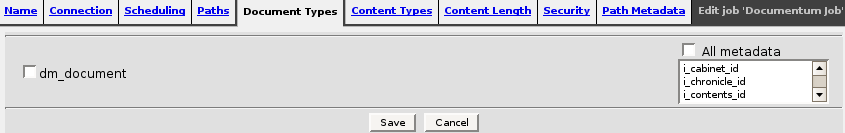
\includegraphics[width=300pt]{Docu-edit-job-tab5}

\begin{itemize}

\item \textbf{Document Types:} Select here the Documentum document
subclasses you wish to include in your job. Simply check the
subclasses you wish to include. The list of document subclasses is
generated by your Documentum repository based on existing document
subclasses.

\item \textbf{Metadata:} The Documentum repository stores various
metadata information about documents in its index.  You can select
those metadata fields here and have them sent along with the files you
index as metadata.  Each document subclass has its own selection box,
listing the metadata fields available for that particular
subclass. You can select ranges using the Shift key and make multiple
selections using the Ctrl key.  Metadata will not be geographically
parsed or used to create the index on the MetaCarta appliance;
however, with the standard MetaCarta Search APIs, you can construct
searches based specifically on this metadata. For more information on
the SOAP Search API, please see the \documentref{MetaCarta SOAP Search
API Guide}. For more information on the JSON Search API and KML Search
API, please see the \documentref{MetaCarta Guide to Web Services
Search APIs}.

\end{itemize}

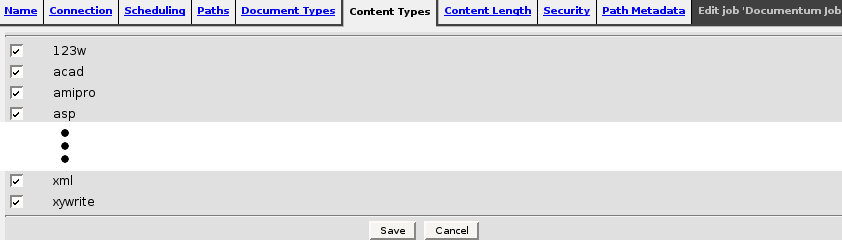
\includegraphics[width=300pt]{Docu-edit-job-tab6}

\begin{itemize}

\item \textbf{Content Types:} Here you can select the Documentum
content types you wish this job include. This list of Documentum
content types is generated by your Documentum repository based on the
content types present in the system. These content types will not
correspond directly with the filetypes supported by MetaCarta;
however, the supported filetypes provide a rough guideline for the
types of content that can be ingested.

\input{supported}

Some content types are easily matched to filetypes; for example the
content type \command{html} corresponds to HTML documents, and the
content type \command{pdf} corresponds to Adobe Acrobat
files. Other relationships may not be as clear. The content types
\command{msw}, \command{msw3}, \command{msw6}, \command{msw8},
\command{mwsm}, \command{mswm1}, and \command{msww} all correspond to
Microsoft Word documents, while the content type
\command{doc} corresponds to an Interleaf\circler\ 3.x or 4.x
file. Your Documentum installation includes a full list of the default
content types and their formats at
\dirpath{%DM_HOME%/install/tools/formats.csv}. See your Documentum
documentation for more details.

If documents of a given content type cannot be ingested they will not
be indexed by the appliance.

\end{itemize}

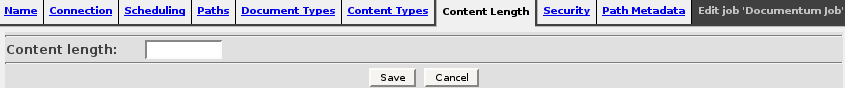
\includegraphics[width=300pt]{Docu-edit-job-tab7}

\begin{itemize}

\item \textbf{Content Length:} The maximum file size, in bytes, that
you wish this job to crawl. Files larger than this size will be
skipped. The default maximum content length is unlimited. 

\end{itemize}


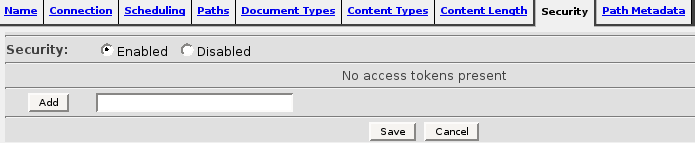
\includegraphics[width=300pt]{Docu-edit-job-tab8}

\begin{itemize}

\item \textbf{Security:} Use this option to enable or disable document
security. If you choose to enable security, user permissions will be
ingested with documents, while if you choose to disable security,
documents will be ingested without permissions.

\item \textbf{Access Tokens:} \label{ForceACL} If you wish to specify
your own ACLs for files ingested through this job, you can specify
them here. You should use this option if you selected ``Standard
(Kerberos)'' as the authority connection for your repository
connection and you are choosing to enable security. Simply enter one
or more ACL identifiers into the field and click the ``Add''
button. The ACL identifiers will appear in a list. You can continue to
add more ACL identifiers using the ``Add'' button, or remove them
using the ``Delete'' button that appears next to each ACL identifier.

\end{itemize}

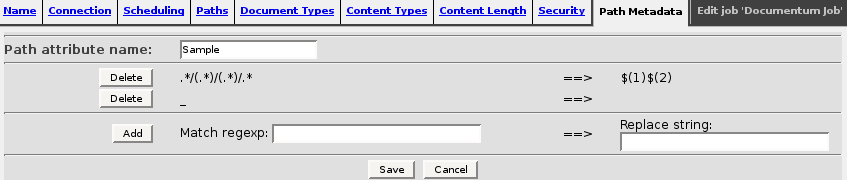
\includegraphics[width=300pt]{Docu-edit-job-tab9}

\begin{itemize}

\item \textbf{Path Attribute name:} The name for the metadata field
representing path attributes. This should be a recognizable name
distinct from any of the metadata fields already associated with any
document type being ingested. It may be useful to have the metadata
field containing path attributes have the same name across jobs.

\item \textbf{Path-value mapping:}The regular expressions and
substitutions that you want to use to collect information from the
Documentum file path. You can construct one or more regular
expressions. In the example shown, there are two expressions. The
first, \verb+.*/(.*)/(.*)/.*+ to \verb+$(1) $(2)+, would change the
directory path ``Project/Folder\_1/Folder\_2/ Filename'' into
``Folder\_1 Folder\_2.'' The second, \_ to a space, would then be
applied to turn the metadata into ``Folder 1 Folder 2.'' It is
important to allow more than one transform so that you can, if
necessary, extract text data and then parse the extracted data. The
end result of the last transform will be ingested as the value of the
metadata attribute defined previously. For more information on regular
expressions, see the note on page \pageref{regex}.

\end{itemize}


After entering this information, you will be taken to the status page
for this job:

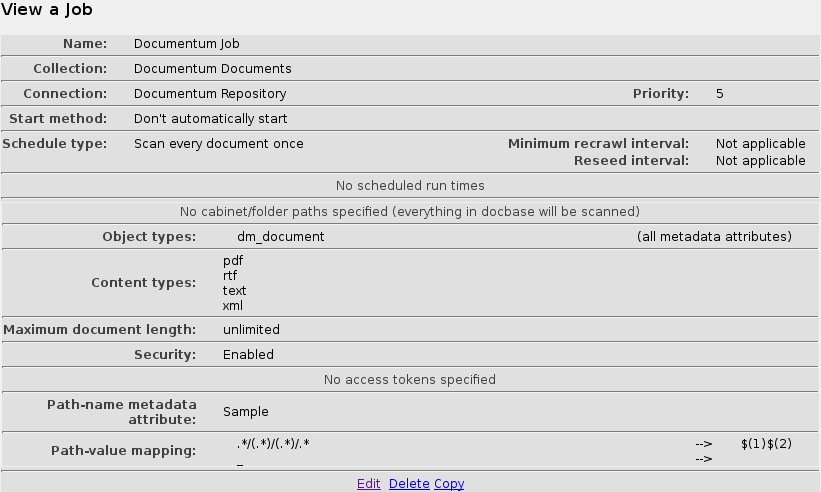
\includegraphics[width=300pt]{Docu-view-job-status}



% Licensed to the Apache Software Foundation (ASF) under one or more
% contributor license agreements. See the NOTICE file distributed with
% this work for additional information regarding copyright ownership.
% The ASF licenses this file to You under the Apache License, Version 2.0
% (the ``License''); you may not use this file except in compliance with
% the License. You may obtain a copy of the License at
%
% http://www.apache.org/licenses/LICENSE-2.0
%
% Unless required by applicable law or agreed to in writing, software
% distributed under the License is distributed on an ``AS IS'' BASIS,
% WITHOUT WARRANTIES OR CONDITIONS OF ANY KIND, either express or implied.
% See the License for the specific language governing permissions and
% limitations under the License.

\subsubsection{JDBC Job Options}

You must fill in the ``Scheduling,'' ``Queries,'' and ``Security''
tabs to configure a JDBC job.

\bigimage{JDBC-edit-job-tab3}

\ifJDBCGuide
\input{schedule-input}
\fi

\ifCombinedConnectorGuide
This tab presents scheduling options. Here you can generate one or
more scheduled run times for the job. For a complete description of
the scheduling options, see the description starting on page
\pageref{scheduling}.
\fi

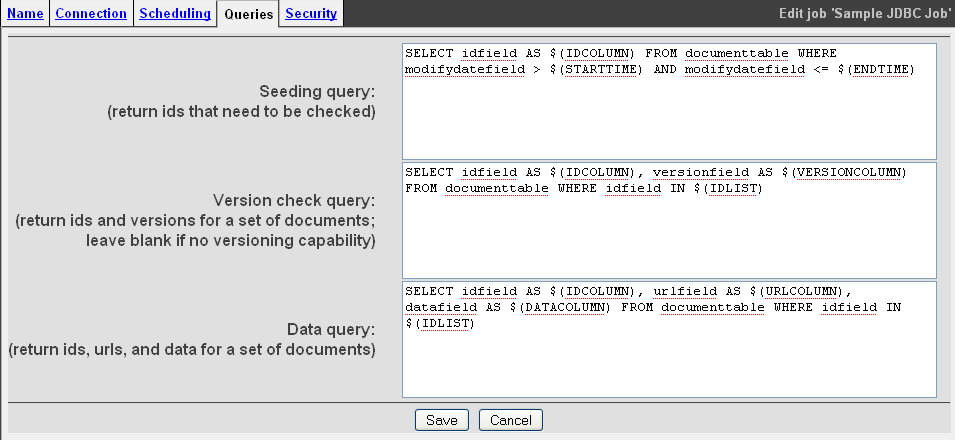
\includegraphics[width=300pt]{JDBC-edit-job-tab4}

In each of the three fields, you will need to construct an appropriate
SQL query. The sample queries shown include helper strings of the form
\command{\$(HELPER)} used by the connector, which are explained as they
appear.

\begin{itemize}

\item \textbf{Seeding Query:} The seeding query should return the
identifiers of documents in the repository that should be checked
against the files indexed in the GTS database. These identifiers
should be returned in a result-set as a column named
\command{\$(IDCOLUMN)}. The sample query shown above reads:

\begin{console}
SELECT idfield AS \$(IDCOLUMN) FROM documenttable WHERE modifydatefield
> \$(STARTTIME) AND modifydatefield <= \$(ENDTIME)

\end{console}

In this sample seeding query, identifiers from \command{idfield} for
entries from table \command{documenttable} are returned as a column
named \command{\$(IDCOLUMN)}. This example uses a \command{WHERE}
expression to limit the returned identifiers to entries with a
modified date, \command{modifydatefield}, in the range specified by
\command{\$(STARTTIME)} to \command{\$(ENDTIME)}. The time range spans
from the last time the job was run to the current start time, as
maintained by the GTS appliance. Time filtering is not a required part
of this query, but it helps reduce the number of documents being
passed to the ingestion interface by filtering out documents that have
not been modified since the last time the job was run.

A seeding query must be included. The seeding query must return a
column named \command{\$(IDCOLUMN)} as part of its result-set.

\note{Use caution when constructing queries that include time-based
components. \command{\$(STARTTIME)} and \command{\$(ENDTIME)} provide
times in milliseconds since epoch. If the modified date field is not
in this unit, the seeding query may not select the desired document
identifiers. You should convert \command{\$(STARTTIME)} and
\command{\$(ENDTIME)} to the appropriate timestamp unit for your system.

The following table gives several sample query fragments that can be
used to convert the helper strings \command{\$(STARTTIME)} and
\command{\$(ENDTIME)} into other date and time types. The first column names
the SQL database type that the following query phrase corresponds to,
the second column names the output data type for the query phrase, and
the third gives the query phrase itself using \command{\$(STARTTIME)}
as an example time in milliseconds since epoch. These query phrases
are intended as guidlines for creating an appropriate query phrase in
each language. Each query phrase is designed to work with the most
current version of the database software available at the time of
publishing for this document. If your modified date field is not of
the type given in the second column, the query phrase may not provide
an appropriate output for date comparisons.}

\input{sql-time-queries}

\item \textbf{Version Check Query:} If your document system has
versioning capabilities, a version check query should be used to
filter documents based on version. The sample version query shown
above reads:

\begin{console}
SELECT idfield AS \$(IDCOLUMN), versionfield AS \$(VERSIONCOLUMN) FROM
documenttable WHERE idfield IN \$(IDLIST)
\end{console}

The sample query returns a column
named \command{\$(IDCOLUMN)} of identifiers from \command{idfield} and a
column named \command{\$(VERSIONCOLUMN)} of version numbers from
\command{versionfield} from entries in the table \command{documenttable}
whose identifiers were passed to this query by the job process using
the input \command{\$(IDLIST)}.

A version check query is not required. If your document system does
not have versioning capability, leave this query blank.

\item \textbf{Data Query:} A data query returns the identifiers, URLs,
and data for a document. The sample data query shown above reads:

\begin{console}
SELECT idfield AS \$(IDCOLUMN), urlfield AS \$(URLCOLUMN), datafield AS
\$(DATACOLUMN) FROM documenttable WHERE idfield IN \$(IDLIST)
\end{console}

This sample data query returns three columns, a column named\linebreak
\command{\$(IDCOLUMN)} of identifiers from \command{idfield}, a column
named \command{\$(URLCOLUMN)} of document URLs from \command{urlfield},
and a column named \command{\$(DATACOLUMN)} of document contents from
\command{datafield}. These outputs are generated from entries in the table
\command{documenttable} whose identifiers were passed to this query by
the job process using the input \command{\$(IDLIST)}.

The data query is required. This query passes the documents and
associated information to the ingestion interface for either initial
ingestion or re-ingestion.

\end{itemize}

When possible, filter the files passed to the ingestion interface by
way of version, modification time, or other methods to reduce the
number of files that are re-ingested unnecessarily. This can
significantly improve the performance of the ingestion.

The exact entry form of helper strings varies depending on the type of
database being used. In the case of Postgres SQL, MS SQL Server, and
Sybase, the helper strings should just be entered as shown in the
sample queries, as \command{\$(HELPER)}. In the case of Oracle, the
helper strings naming columns should be enclosed in double
quotation marks, as \command{\char34\$(IDCOLUMN)\char34},
\command{\char34\$(VERSIONCOLUMN)\char34},\linebreak
\command{\char34\$(URLCOLUMN)\char34}, and
\command{\char34\$(DATACOLUMN)\char34}, while the helper strings
\command{\$(IDLIST)}, \command{\$(STARTTIME)}, and
\command{\$(ENDTIME)} should be left as shown.

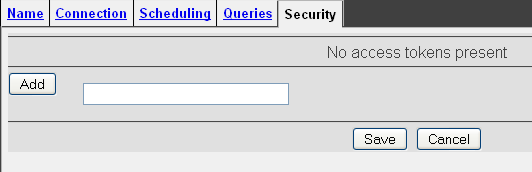
\includegraphics[width=300pt]{JDBC-edit-job-tab5}

If you wish to enable security, the user permissions you enter here will
be ingested with each document in this job. Otherwise, all documents in
this job will be ingested without permissions.

\item \textbf{Access Tokens:} To specify your own ACLs for files ingested
through this job, you can specify enter one or more ACL identifiers into
this field and click the ``Add'' button. The ACL identifiers will appear
in a list. You can continue to add more ACL identifiers using the ``Add''
button, or remove them using the ``Delete'' button that appears next to
each ACL identifier.

After entering this information, you will be taken to the status page
for this job:

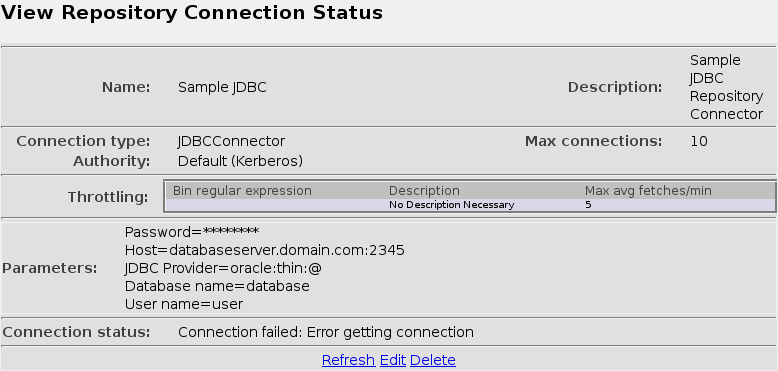
\includegraphics[width=300pt]{JDBC-view-job-status}


% Licensed to the Apache Software Foundation (ASF) under one or more
% contributor license agreements. See the NOTICE file distributed with
% this work for additional information regarding copyright ownership.
% The ASF licenses this file to You under the Apache License, Version 2.0
% (the ``License''); you may not use this file except in compliance with
% the License. You may obtain a copy of the License at
%
% http://www.apache.org/licenses/LICENSE-2.0
%
% Unless required by applicable law or agreed to in writing, software
% distributed under the License is distributed on an ``AS IS'' BASIS,
% WITHOUT WARRANTIES OR CONDITIONS OF ANY KIND, either express or implied.
% See the License for the specific language governing permissions and
% limitations under the License.

\subsubsection{Livelink Job Options}

In the Livelink-specific tabs, you will have the following additional
settings:

\bigimage{edit-job-tab3}

\ifLivelinkGuide
\input{schedule-input}
\fi

\ifCombinedConnectorGuide
This tab presents scheduling options. Here you can generate one or
more scheduled run times for the job. For a complete description of
the scheduling options, see the description starting on page
\pageref{scheduling}.
\fi

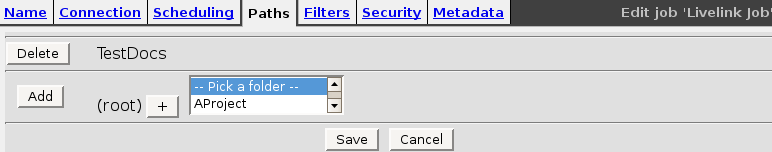
\includegraphics[width=300pt]{edit-job-tab4}

\begin{itemize}

\item \textbf{Roots:} The base directories in Livelink from which you
want your crawl to start. You may select zero, one, or more than one
(though if you select zero, your appliance will not crawl anything). 
To select a directory, select the directory name, click the ``+''
button, and then click ``Add.'' The directory will appear inside the selection
box; you can click the ``Delete'' button next to it to remove it from
your list of directories to be crawled.

\end{itemize}

\includegraphics[width=300pt]{edit-job-tab5}

\begin{itemize}

\item \textbf{Filters:} You must define the files that will be 
crawled and indexed during this job. You do this by specifying filetypes
of the form ``\*.XYZ.'' You must specify at least one filetype to 
include, or you will not crawl any documents.

For example, if you want to crawl .QZX
files, you can enter ``\*.QZX'', select ``Include'', and then click Add.
You may define multiple inclusions and exclusions; if an exclusion and an
inclusion conflict, the first one you entered is followed.  

\input{supported}

To crawl and index all files, enter ``\*.\*'' and click Add.

\end{itemize}

\includegraphics[width=300pt]{edit-job-tab6}

\begin{itemize}

\item \textbf{Security:} Allows you to control whether or not file ACLs,
or access control lists, are passed to the appliance with the files. If
you select ``Disabled'' here, all files crawled from Livelink will be
visible to all GTS users.

\item \ifLivelinkGuide \label{ForceACL}\fi \textbf{Access Tokens:} If you want to pass on
your own Active Directory ACLs instead of those used by Livelink---or
your Livelink instance does not contain Livelink ACLs---you can enter
them here.  You should enter one or more SIDs that you want to have
read permissions on the files crawled in this job. Two special
Livelink tokens can also be entered. The token ``SYSTEM'' represents
Livelink system administrators, while the token ``GUEST'' represents
users logged into Livelink as guests. For more information about AD
ACLs and SIDs, please see the security sections of the
\documentref{MetaCarta Appliance Administrator's Guide}.

\note{If you have disabled security, these ACLs will not be passed to
the appliance.}

\end{itemize}

\includegraphics[width=300pt]{edit-job-tab7}

\begin{itemize}

\item \textbf{Ingest ALL metadata:} Choose yes if you want to ingest all 
metadata for each document crawled.

\item \textbf{Metadata:} The Livelink server stores various metadata
information about documents in its index.  You can select those metadata
fields here and have them sent along with the files you index as metadata.
Metadata will not be geographically parsed or used to create the index
on the MetaCarta appliance; however, with the SOAP Search API, you
can construct searches based specifically on this metadata. For more
information on the SOAP Search API, please see the \documentref{MetaCarta
SOAP Search API Guide}.

\item \textbf{Path attribute name:} The name of the GTS metadata
attribute to which you want to attach Livelink file path data, if any.

\item \textbf{Path-value mapping:} The regular expressions
and substitutions that you want to use to collect information
from the Livelink file path. Using the regular expression
rules on page \pageref{regex}, you can construct one or more
expressions. In the example shown, there are two expressions. The
first, \verb+.*/(.*)/(.*)/.*+ to \verb+$(1) $(2)+, would change the
directory path ``Project/Folder\_1/Folder\_2/ Filename'' into ``Folder\_1
Folder\_2.'' The second, \_ to a space, would then be applied to turn
the metadata into ``Folder 1 Folder 2.'' It is important to allow more
than one transform so that you can, if necessary, extract text data and
then parse the extracted data. The end result of the last transform will
be ingested as the value of the metadata attribute defined previously.

\end{itemize}

After entering this information, you will be taken to the status page
for this job:

\includegraphics[width=300pt]{view-job-status}


% Licensed to the Apache Software Foundation (ASF) under one or more
% contributor license agreements. See the NOTICE file distributed with
% this work for additional information regarding copyright ownership.
% The ASF licenses this file to You under the Apache License, Version 2.0
% (the ``License''); you may not use this file except in compliance with
% the License. You may obtain a copy of the License at
%
% http://www.apache.org/licenses/LICENSE-2.0
%
% Unless required by applicable law or agreed to in writing, software
% distributed under the License is distributed on an ``AS IS'' BASIS,
% WITHOUT WARRANTIES OR CONDITIONS OF ANY KIND, either express or implied.
% See the License for the specific language governing permissions and
% limitations under the License.


\subsubsection{Share Job Options}

You must complete the following tabs to configure a Share Job:

\bigimage{Share-edit-job-tab3}


\ifShareGuide
\input{schedule-input}
\fi

\ifCombinedConnectorGuide
This tab presents scheduling options. Here you can generate one or
more scheduled run times for the job. For a complete description of
the scheduling options, see the description starting on page
\pageref{scheduling}.
\fi


\includegraphics[width=300pt]{Share-edit-job-tab4}

\begin{itemize}

\item \textbf{Paths:} Here you can specify directory and file paths in
your network share from which you want your crawl to start. You can
specify one or more paths. If you do not specify any paths, the job
will not crawl any directories or documents. To generate each set of
paths, you must first build a directory path. You can build a
directory path by selecting individual directories. To start, you can
either select the base directory from the selection box or, if it does
not appear in the selection box, type its name in the empty text box,
then click the ``+'' button. A new selection box will appear with the
directories contained by that parent directory, along with a new text
box. Select or fill in a directory at that level and click the ``+''
button. Continue building your directory path in this fashion. When
it's complete, click ``Add''.

The directory path will appear along with a crawl customization
box. Using this customization box, you can use Windows file matching
expressions (or ``wildcard expressions'') to further specify directory and
file paths to crawl. Each path customization includes three parts. The
first selection is used to include or exclude items matched by a
wildcard expression. The second selection allows you to specify what
types of files and/or directories should be included with this
customization. The last part is a text box in which you can enter a
wildcard expression used to match files and/or directories. Complete
all three fields and click ``Add'' to insert the wildcard expression
instruction at the end of the list of instructions.

The list of wildcard expression instructions is evaluated from top to
bottom. Customization boxes appear in between list items, allowing the
insertion of instructions into the list. A wildcard expression
instruction can be deleted from the list by clicking the ``Delete''
button that appears next to it. By default, the list of instructions
includes two statements, \command{1.~Include file(s) matching *} and
\command{2.~Include directory(s) matching *}. Together these
instructions tell the job to crawl all contents contained by the
parent directory path.

Wildcard expressions use wildcard characters to match file and
directory names. The character \texttt{*} is used to match any zero or
more characters, while the character \texttt{?} matches any single
character. The brackets characters \texttt{[]} match any single
selection of characters that appears within the brackets. Simply
entering \texttt{*} as an expression matches everything. Some other
possiblities:

\begin{itemize}

\item \texttt{file??.txt}: A sequence of text files with a two digit
identifier.

\item \texttt{file*.txt}: A sequence of text files with a variable
length identifier.

\item \texttt{*.txt}: Any text file.

\item \texttt{*Data}: Any directory whose name ends with the word
``Data''.

\item \texttt{[abc]*}: Any file or directory whose name begins with
``a'', ``b'', or ``c''.

\item \texttt{*.[abc]*}: Any file whose extension begins with ``a'',
``b'', or ``c''.

\end{itemize}

You can continue to add more directory paths to your list using the
new selection box that appears below your completed directory
path. Each directory path can be customized with instructions as
described above. To remove a directory path from the list, click the
``Delete'' button next to it.

\end{itemize}

\includegraphics[width=300pt]{Share-edit-job-tab5}

\begin{itemize}

\item \textbf{File Security:}  Allows you to control whether or not file ACLs,
or access control lists, are passed to the appliance with the files.

\item \textbf{Access Tokens:} If you want to pass on your own Active
Directory ACLs instead of those of the network share you can enter
them here. You should enter one or more SIDs that you want to have
read permissions on the files crawled in this job. For more
information about AD ACLs and SIDs, please see the security sections
of the \documentref{MetaCarta Appliance Administrator's Guide}.

\note{If you have disabled security, these ACLs will not be passed to
the appliance.}

\item \textbf{Share Security:} In some cases, your network share's
security may include share security. You should enable or disable
share security to match your network share's security model.

\end{itemize}

\includegraphics[width=300pt]{Share-edit-job-tab6}

\begin{itemize}

\item \textbf{Path Attribute name:} You can create a metadata field
to contain attributes from the file path. You can enter a name
for the metadata field here. It may be useful to have the metadata
field containing path attributes have the same name across jobs.
This metadata will not be geographically parsed or used to create the
index on the MetaCarta appliance; however, with MetaCarta Search APIs,
you can construct searches based specifically on this metadata. For more
information on the SOAP Search API, please see the \documentref{MetaCarta
SOAP Search API Guide}, and for more information on the JSON and KML
Search APIs, please see the \documentref{Web Services Search Guide}.

\item \textbf{Path-value mapping:}The regular expressions and
substitutions that you want to use to collect information from the
file path. You can construct one or more regular expressions. In the
example shown, there are two expressions. The first,
\verb+.*/(.*)/(.*)/.*+ to \verb+$(1) $(2)+, would change the directory
path ``Project/Folder\_1/Folder\_2/ Filename'' into ``Folder\_1
Folder\_2.'' The second, \_ to a space, would then be applied to turn
the metadata into ``Folder 1 Folder 2.'' It is important to allow more
than one transform so that you can, if necessary, extract text data
and then parse the extracted data. The end result of the last
transform will be ingested as the value of the metadata attribute
defined previously. \ifCombinedConnectorGuide If you are not familiar
with regular expressions, please see the note on page \pageref{regex}
for more information.\fi

\ifShareGuide 
\label{regex} 

\note{If you are not familiar with regular expressions, there
are a variety of tutorials available on the web, including
\url{http://gnosis.cx/publish/programming/regular_expressions.html}
and \url{http://}\linebreak \url{perldoc.perl.org/perlrequick.html}. If
you still have difficulty with these settings, please contact Customer
Support (see page \pageref{SupportContact}).} 

\fi

\end{itemize}

\includegraphics[width=300pt]{Share-edit-job-tab7}

\begin{itemize}

\item \textbf{Content Length:} The maximum file size, in bytes, that
you wish this job to crawl. Files larger than this size will be
skipped. The default maximum content length is unlimited.


After entering this information, you will be taken to the status page
for this job:

\includegraphics[width=300pt]{Share-view-job-status}


\end{itemize}



% Licensed to the Apache Software Foundation (ASF) under one or more
% contributor license agreements. See the NOTICE file distributed with
% this work for additional information regarding copyright ownership.
% The ASF licenses this file to You under the Apache License, Version 2.0
% (the ``License''); you may not use this file except in compliance with
% the License. You may obtain a copy of the License at
%
% http://www.apache.org/licenses/LICENSE-2.0
%
% Unless required by applicable law or agreed to in writing, software
% distributed under the License is distributed on an ``AS IS'' BASIS,
% WITHOUT WARRANTIES OR CONDITIONS OF ANY KIND, either express or implied.
% See the License for the specific language governing permissions and
% limitations under the License.

\subsubsection{RSS Job Options}

You must fill in six more tabs to configure an RSS job.

\bigimage{RSS-edit-job-tab3}

\ifJDBCGuide
\input{schedule-input}
\fi

\ifCombinedConnectorGuide
This tab presents scheduling options. Here you can generate one or
more scheduled run times for the job. For a complete description of
the scheduling options, see the description starting on page
\pageref{scheduling}.
\fi

RSS feeds that are updated regularly will have documents fall off of the
end of the feed. If you are crawling continuously, those documents will
remain on the appliance until the expiration time set in this tab. If you
are crawling non-continuously, when the RSS connector job runs, documents
that are no longer in the feeds will be deleted from the appliance index.

\bigimage{RSS-edit-job-tab4}

On this tab, you are presented with a text box into which you should
enter the URLs of the feeds you wish this job to crawl. Each should be
on a separate line of the text box.

\bigimage{RSS-edit-job-tab5}

This tab allows you to apply some built-in canonicalization tools
to URLs before they are send to the MetaCarta ingestion system. If
canonicalization is not done properly, you risk either having duplicate
copies of the same document (for example, from having arguments to
a script in a different order but calling the script with the same
arguments) or having no copies of a document at all (for example, from
reordering the script arguments in a way that breaks the site being
crawled). The Connector Framework handles the reordering automatically,
but requires your intervention to decide which sites need to be reordered
and which do not. 

You can canonicalize based on regular expression; for more information on
regular expressions, please see the explanation in the next tab. Enter
a regular expression, a description of the URL (for your records only),
and then choose the types of canonicalization you would like enabled. You
have the following canonicalization options:

\begin{itemize}

\item \textbf{Reorder}: Take all arguments to any query in the URL and
order them programmatically. For example, a URL might include a query
string like ``article=foo0011\&format=fulltext.'' If the query string
were instead ``format=fulltext\&article=foo0011,'' the MetaCarta system
would treat it as a different document but it would contain the same
information. Normally, we recommend that you reorder all URLs, but
some sites require a specific order; for those sites, you should turn
reordering off.

\item \textbf{Remove JSP sessions}: Most of the time, you can safely
remove JSP session information from URLs. Uncheck this box if you find
that a particular site requires that you leave JSP session information
in the URL.

\item \textbf{Remove ASP sessions}: Most of the time, you can safely
remove ASP session information from URLs. Uncheck this box if you find
that a particular site requires that you leave ASP session information
in the URL.

\item \textbf{Remove PHP sessions}: Most of the time, you can safely
remove PHP session information from URLs. Uncheck this box if you find
that a particular site requires that you leave PHP session information
in the URL.

\item \textbf{Remove BV sessions}: Most of the time, you can safely
remove BV session information from URLs. Uncheck this box if you find
that a particular site requires that you leave BV session information
in the URL.

\end{itemize}

By default, all URLs are canonicalized in all five ways. 

\bigimage{RSS-edit-job-tab6}

This tab allows you to manipulate the URL ingested along with a
document. The URL ingested along with a document is by default the URL
from which the document was retrieved, but you may wish to provide a
different URL to be associated with the document. You can use regular
expressions to manipulate the URL. The example regular expression,
\verb+(.*)\:\/\/([A-Z|a-z|0-9|_|-|.]*)\/(.*)+, takes a URL, and breaks
it down into three parts; the protocol, the host server, and the file
path. The replacement string, \verb+1,''://www.example.com'',3+,
substitutes ``www.example.com'' for the host server.

You can specify more than one mapping. The mappings are applied in the
order in which they appear.

\note{If you are not familiar with regular expressions, there
are a variety of tutorials available on the web, including
\url{http://gnosis.cx/publish/}\linebreak\url{programming/regular_expressions.html}
and \url{http://perldoc.}\linebreak\url{perl.org/perlrequick.html}. If you still have
difficulty with these settings, please contact Customer Support (see
page \pageref{SupportContact}).}


\bigimage{RSS-edit-job-tab7}

\begin{itemize}

\item \textbf{Feed connect timeout (seconds):} A document fetch will time out after a period of inactivity. This field allows you to set the length of the timeout interval.

\item \textbf{Default feed refetch time (minutes)}: The feed may provide a suggested refetch interval. If no interval is provided, the crawler will use the interval you provide here.

\item \textbf{Minimum feed refetch time (minutes)}: If the suggested refetch interval is shorter than the interval specified here, the crawler will use this refresh interval.

\item \textbf{Bad feed refetch time (minutes)}: If the suggested refetch interval is shorter than the interval specified here, the crawler will use this refresh interval for bad feeds. 

\end{itemize}

\bigimage{RSS-edit-job-tab8}

\begin{itemize}

\item \textbf{Access Tokens:} If you wish to specify ACLs for files ingested through this job, you can specify them here. Simply enter one or more ACL identifiers into the field and click the ``Add'' button. The ACL identifiers will appear in a list. You can continue to add more ACL identifiers using the ``Add'' button, or remove them using the ``Delete'' button that appears next to each ACL identifier. By default, documents ingested through the RSS Connector will be accessible to all authorized search users. For assistance with this configuration, contact MetaCarta Support (see page \pageref{SupportContact}).

\end{itemize}

\bigimage{RSS-edit-job-tab9}

\begin{itemize}

\item \textbf{Metadata:} Here you can add additional metadata to be ingested along with documents crawled by this job. You should not overwrite existing metadata fields, such as collection name, using this tool.

\end{itemize}

\bigimage{RSS-edit-job-tab10}

Many commercial websites use ``chrome,'' or branding and advertising
information, that presents users with a number of browsing options
from the article they are reading. Unfortunately, this information
is often geographic, and can degrade the accuracy of the MetaCarta
indexing process. To solve this problem, the RSS site administrator
can include a ``dechromed'' version of the article, usually the article
itself without any additional information, in either the ``description''
or the ``content'' field of each article.

You can choose one of these three options:

\begin{itemize}

\item \textbf{No dechromed content:} There is no dechromed content in
this feed; the crawler should just fetch each document.

\item \textbf{Dechromed content, if present, in `description' field:}
The crawler will check the `description' field for content before fetching
the original document, and use anything it finds there preferentially.

\item \textbf{Dechromed content, if present, in `content' field:}
The crawler will check the `content' field for content before fetching
the original document, and use anything it finds there preferentially.

\end{itemize}

You can choose one of these two options:

\begin{itemize}

\item \textbf{Use chromed content if no dechromed content found:} If
there is no dechromed content, fetch the original document.

\item \textbf{Never use chromed content:} If there is no dechromed content,
do not index this document at all.

\end{itemize}

After entering this information, you will be taken to the status page
for this job:

\includegraphics[width=300pt]{RSS-view-job-status}


\subsection{Status and Job Management}\label{ManageJobs}

You can then look at the status of your job by clicking ``Status and 
Job Management'' on the sidebar. You will see a list of one or more jobs
much like this one:

\includegraphics[width=300pt]{Generic-jobs-list}

You can start any crawl you like immediately from this interface by
clicking ``Start'' next to the crawl's name. This interface also allows
you to see how many documents have been crawled; this information may help
you structure and plan future crawls. ``Active'' documents are currently
known documents that will need to be processed during the current job run.
``Processed'' documents have been processed at least once, in the current
run or previous runs.

\note{Refresh this page by clicking the ``Refresh'' link at the bottom
of the page, not by clicking your browser's reload button.}

\section{Reports}

The Connector Framework interface can generate two types of status
reports, or reports on the current crawl status, and four types of
history reports, reports on crawls already going on. The six types are:

\begin{itemize}

\item Document Status, which lets you find information on individual 
documents currently part of a job 

\item Queue Status, which lets you aggregate information about groups
of documents currently part of a job 

\item Simple History, which lets you list an ordered set of log events
based on chosen criteria

\item Maximum Activity, which lets you see the period of time in
which a certain event happened most often

\item Maximum Bandwith, which lets you see the period of time in
which the most bandwidth was used 

\item Result Histogram, which provides log information that would be
appropriate for constructing a histogram or other diagram

\end{itemize}

\subsection{Status Reports}


\subsubsection{Document Status}

This report was generated by selecting ``MetaCarta Sample,'' selecting
the document state ``Documents processed at least once,'' selecting all 
possible document statuses, clicking continue, selecting ``Sample Job,''
and clicking Go.

\includegraphics[width=300pt]{Generic-document-report}

\begin{itemize}

\item \textbf{Connection:} The repository connection from which to 
generate a report. You must select the repository connection and click
Continue to see all repository-specific options. %Are there any?

\item \textbf{Time offset from now:} Defaults to zero. Allows you to
see estimates of future status or, with negative numbers, a record of
past status.

\item \textbf{Document state:} Allows you to select documents that
have not yet been processed or documents that have been processed
at least once.

\item \textbf{Document status:} Allows you to choose one or more 
statuses of document to report on. The statuses you can choose are:

\begin{itemize}

\item Documents that are no longer active

\item Documents currently in progress

\item Documents currently being expired

\item Documents currently being deleted

\item Documents currently available for processing

\item Documents currently available for expiration

\item Documents not yet processable

\item Documents not yet expirable

\end{itemize}

\item \textbf{Document identifier match:} A regular expression allowing
you to see only certain document identifiers.

\item \textbf{Jobs:} The job or jobs for which you want to generate
a report.

\end{itemize}

You can sort this report by any of the returned fields; to do so,
click the field names.

\subsubsection{Queue Status}

This report was generated by selecting ``MetaCarta Sample,'' selecting
the document state ``Documents processed at least once,'' selecting all
possible document statuses, clicking continue, selecting ``Sample Job,''
setting the identifier class description to (/9/9/9), and clicking Go.

\includegraphics[width=300pt]{Generic-queue-report}

This form offers the same fields as the Document Status report with
one addition, the \textbf{Identifier class description}, which allows
you to group results based on a regular expression. In this case, any
document whose path contains ``/9/9/9'' is collected into a group, and
that group's documents are analyzed  separately from the other documents
selected. The ungrouped documents are all analyzed together in the first
row of the results table. If the identifier class description were just
``.*'' then each document would be shown individually as a group of one.

\subsection{History Reports}

Each of these reports allows you to specify a connection, one or more
activities, a start time, an end time, an entity match, and a result code
match.  Some also allow you to specify an identifier class description
and a sliding window size. This section will show sample results for
each type of report and an explanation of the fields selected.

\subsubsection{Simple History}

This report was generated by selecting ``Sample Repository Connector,'' 
clicking Continue, selecting ``document ingest,'' and clicking Go.

\includegraphics[width=300pt]{Generic-simple-history-report}

\begin{itemize}

\item \textbf{Connection:} The repository connection from which to
generate a report. You must select the repository connection and click
Continue to see all repository-specific options.

\item \textbf{Activities:} What crawler activities you would like to
see.  The basic set of activites that can be documented in reports for
all repository connections are document ingest, document remove, job
abort, job continue, job end, job start, and job wait. Some activities
are repository connection-specific:

\begin{itemize}

\item \textbf{Documentum:} fetch

\item \textbf{Livelink:} fetch document, find documents

\item \textbf{Share:} access

\end{itemize}

\item \textbf{Start time:} The earliest time in the crawler logs to be
considered for this query.  Choose ``Not specified'' for any field to
start at the beginning of the crawler's logs.

\item \textbf{End time:} The latest time in the crawler logs to be
considered for this query. Choose ``Not specified'' for any field 
to end at the current time.

\item \textbf{Entity match:} A regular expression (see page
\pageref{regex}) to limit the Identifier field. If the entity match
field in the example above had been \texttt{\^{}17}, only document
fetches with Identifiers starting with 17 would be shown.

\item \textbf{Result code match:} A regular expression to limit the
ResultCode field.

\end{itemize}

You can sort the history report by any of the returned fields; to do so,
click the field names.


\subsubsection{Maximum Activity}

This report was generated by selecting ``Sample Repository Connector,''
clicking Continue, selecting ``document ingest,'' changing the Identifier
class description, and clicking Go.

\includegraphics[width=300pt]{Docu-maximum-activity-report}

This form offers two more fields than the previous form:

\begin{itemize}

\item \textbf{Identifier class description:} A regular expression
that determines how to group identifiers together. If this were set to
\texttt{(.*)}, there would be no grouping, and so there would be only one
ingestion event per document. If this were set to \texttt{(17)},
then all documents with identifiers beginning with 17 would be grouped
together. The setting in the example, \texttt{()}, groups all
documents together. Some other possibilities:

\begin{itemize}

\item \texttt{1(.)}: (up to) Ten groups of documents whose identifier starts
with 1, labeled 0-9, grouped by the second digit of their identifier.

\item \texttt{()}: One group of documents containing all documents 
regardless of identifier.

\item \texttt{17}: One group of documents whose identifier contains
the string ``17.''

\item \texttt{\^{}17}: One group of documents whose identifier \emph{starts}
with the string ``17.''

\end{itemize}

Document identifiers vary from repository to repository. For Documentum
and Livelink repositories, the unique part of the document identifier will
simply be a number. Documentum uses a hexadecimal document identifier,
while Livelink uses standard base 10 integers as document identifiers. For
network shares accessed using the Share Connector, a document identifier
is typically the document's path. For SQL databases accessed using
the JDBC Connector, the document identifier is set in the database and
can take any form as specified in the database.

\item \textbf{Sliding window size}: The search interval in minutes.

\end{itemize}

The report returned will have only one result per group with one or more
documents in it, if there is a clear highest activity rate, or a list of
all the results tied for highest activity rate if there are more than one.

\subsubsection{Maximum Bandwidth}

This report was generated by selecting ``Sample Repository Connector,''
clicking Continue, selecting ``document ingest,'' changing the Identifier
class description, and clicking Go.

\includegraphics[width=300pt]{Generic-maximum-bandwidth-report}

This form offers the same fields as the maximum activity form, and
returns similar results; instead of tracking events per time window,
it tracks the window with the highest average bandwith usage, measured
in bytes per second. Again, the identifier class description has been
changed to a regular expression that will match all identifiers (and
thus in this case documents).

\subsubsection{Result Histogram}

This report was generated by selecting ``Sample Repository Connector,''
clicking Continue, selecting ``document ingest,'' and clicking Go.

\includegraphics[width=300pt]{Generic-activity-result-report}

This form adds one new field:

\begin{itemize}

\item \textbf{Result code class description:} A regular expression that
determines how to group result classes together; like Identifier class
descriptions but for result classes.

\end{itemize}

This report does not produce an actual histogram, but provides data that
could be used to generate histograms.  

\section{Troubleshooting}

If you see the following error message, or a similar error message:

\includegraphics[width=300pt]{no-mucking-error}

then it is likely that your appliance is part of a Standby Appliance
pair. If your appliance is a standby appliance, this error is expected;
you should make configuration changes only on the primary appliance.
If your appliance is a primary appliance, this message should mean either
that your standby appliance is down and your primary appliance will
not allow the ingestion of new documents or changing of configuration,
or that your primary appliance is in the process of being paired to
a standby appliance. Contact your appliance administrator, or read
the Standby Appliance section of the \documentref{MetaCarta Appliance
Administrator's Guide}, for more information.

If you see this error message while not part of a Standby
Appliance pair, please contact Customer Support (see page \pageref{SupportContact}).

\end{changemargin}



% The SLB/MC Support information must be at the end of every document.
% We include it here, and use \include so that we get the pagebreak.
% Apache will want to change this.
% Licensed to the Apache Software Foundation (ASF) under one or more
% contributor license agreements. See the NOTICE file distributed with
% this work for additional information regarding copyright ownership.
% The ASF licenses this file to You under the Apache License, Version 2.0
% (the ``License''); you may not use this file except in compliance with
% the License. You may obtain a copy of the License at
%
% http://www.apache.org/licenses/LICENSE-2.0
%
% Unless required by applicable law or agreed to in writing, software
% distributed under the License is distributed on an ``AS IS'' BASIS,
% WITHOUT WARRANTIES OR CONDITIONS OF ANY KIND, either express or implied.
% See the License for the specific language governing permissions and
% limitations under the License.

\ifBigMargins\begin{changemargin}{1.5in}{0in}\fi
\ifLittleMargins\begin{changemargin}{.75in}{0in}\fi

\section{Customer Support Contact Information \label{SupportContact}}

Support information goes here.

\end{changemargin}

\end{document}

